\documentclass[a4paper]{report}
\usepackage{hyperref}
\usepackage{parskip}
\usepackage{graphicx}
\usepackage{a4wide}
\usepackage{wrapfig}
\usepackage{subfig}
\usepackage{groove2tikz}
%\usepackage{pdftex}
\usepackage{epstopdf}
\usepackage[all]{xy}
\usepackage{mathtools}
\usepackage{amssymb}
%\usepackage{multirow}
\usepackage{array}

\graphicspath{{./img/}}
%\renewcommand*\familydefault{\sfdefault}

\hypersetup{pdfborder = {0 0 0 0}}

\begin{document}
	\title{\textbf{Model-Based Testing with Graph Transformation Systems}}
	\author{Vincent de Bruijn}
	\date{\today}
	\maketitle
	
	\begin{abstract}
\textit{Graph Grammars} have many structural advantages, which are potential benefits for the model-based testing process. We describe a model-based testing setup with Graph Grammars. The result is a system for automatic test generation from Graph Grammars. A graph transformation tool, GROOVE, and a model-based testing tool, ATM, are used as the backbone of the system. The system is validated using the results of several case-studies.
\end{abstract}

	
	\newpage
	\tableofcontents
  \newpage
  
  \newpage
	\chapter{Introduction}
	\newpage
	%In this introduction, first the importance of testing and automation of testing is stressed. Then Model-Based Testing is shown to be a useful tool for automation of testing. Graph Grammars and graph transformation are argued to be useful as formalism for Model-Based Testing. Some leading tools for automatic test generation are set out, which include the tools used in this report. The research goals are given and finally a roadmap explains the basic structure of the rest of this report.

\section{Testing}
In software development projects, often time and budget costs are exceeded. Laird and Brennan~\cite{Laird:SoftwareMeasurement} investigated in 2006 that 23\% of all software projects are canceled before completion. Furthermore, of the completed projects, only 28\% are delivered on time with the average project overrunning the budget with 45\%. The cause of this often are the unclear ambigious requirements of the software system to develop.

Testing is an important part of software development, because it decreases future maintainance costs~\cite{McConnell:testing}. Testing is a complex process and should be done often~\cite{Pol:testing}. Therefore, the testing process should be as efficient as possible in order to save resources.

Test automation allows repeated testing during the development process. The advantage of this is that bugs are found early and can therefore be fixed early.  A widely used practice is maintaining a \textit{test suite}, which is a collection of test-cases. However, when the creation of a test suite is done manually, this still leaves room for human error~\cite{Blackburn:testing}. The process of deriving tests tends to be unstructured, barely motivated in the details, not reproducible, not documented, and bound to the ingenuity of single engineers~\cite{Utting:MBTTaxonomy}.

\section{Model-based Testing}
The existence of an artifact that explicitly encodes the intended behaviour can help mitigate the implications of these problems. Creating an abstract representation or a \textit{model} of the system is an example of such an artifact. What is meant by a model in this report, is the description of the behavior of a system. In particular, the term model will be often used to describe transition-based notations, such as finite state machines, labelled transition systems and I/O automata. Other notations, such as UML statecharts, are not considered as models in this report. 

A model can be used to systematically generate tests for the system. This is referred to as \textit{model-based testing}. Generating tests automatically leads to a larger test suite than if done manually. A large, systematically built test suite is bound to find more bugs than a smaller, manually built one.

Models are created from the specification documents provided by the end-user. These specification documents are `notoriously error-prone'~\cite{McCabe:testing}. This implies that the model itself needs validation. Validating the model usually means that the requirements themselves are scrutinised for consistency and completeness~\cite{Utting:MBTTaxonomy}. This helps to clear up ambigious requirements early on, which allows better estimation of the budget and time demands.

The stakeholders evaluate the constructed model to verify its correctness. However, the visual or textual representation of large models may become troublesome to understand, which is referred to as the model having a low model transparency or high model complexity. The problem with transition systems is that a larger number of states and/or transitions decreases the model transparency. We think that low model transparency make errors harder to detect and that it obstructs the feedback process of the stakeholders. Using models with high transparency is therefore essential.

\section{Graph Transformation}
A formalism that claims to have more model transparency is Graph Transformation. The system states are represented by graphs and the transitions between the states are accomplished by applying graph change rules to those graphs. These rules can be expressed as graphs themselves. A graph transformation model of a software system is therefore a collection of graphs, each a visual representation of one aspect of the system. This formalism may therefore provide a more intuitive approach to system modelling than traditional state machines. Graph Transformation and its potential benefits have been studied since the early '70s. The usage of this computational paradigm is best described by the following quote from Andries et al.~\cite{Andries1999}: \begin{quote}Graphs are well-known, well-understood, and frequently used means to represent system states, complex objects, diagrams, and networks, like flowcharts, entity-relationship diagrams, Petri nets, and many more. Rules have proved to be extremely useful for describing computations by local transformations: Arithmetic, syntactic, and deduction rules are well-known examples.\end{quote} An informative paper on graph transformations is written by Heckel et al.~\cite{Heckel2006187}. A quote from this paper: \begin{quote}Graphs and diagrams provide a simple and powerful approach to a variety of problems that are typical to computer science in general, and software engineering in particular.\end{quote}

\section{Tools}
Tools for automatic test generation already exist. In Utting et al.~\cite{Utting:MBTTaxonomy}, a taxonomy is done on different model-based testing tools:
\begin{itemize}
  \item TorX~\cite{Tretmans:TorX}: accepts behaviour models such as I/O labelled transition systems. A version of this tool written in Java under continuous development is JTorX~\cite{Belinfante:JTorX}. This version accepts the same kind of models as ATM.
  \item Spec Explorer\cite{Veanes:SpecExplorer}: provides a model editing, composition, exploration and visualization environment within Visual Studio, and can generate offline .NET test suites or execute tests as they are generated (online).
  \item JUMBL\cite{Prowell:JUMBL}: an academic model-based statistical testing that supports the development of statistical usage-based models using Markov chains, the analysis of models, and the generation of test cases.
  \item AETG\cite{Cohen:AETG}: implements combinatorial testing, where the number of possible combinations of input variables are reduced to a few `representative' ones.
  \item STG tool\cite{clarke:STG}: implements conformance testing techniques to automatically derive symbolic test cases from formal operational specifications.
\end{itemize}

The testing tool developed by Axini\footnote{http://www.axini.nl/} is used for the automatic test generation on \textit{symbolic} models, which combine a state and data type oriented approach. This tool is referred to as Axini Test Manager (ATM) and is used in practice by several Dutch companies.

The choice was made to use ATM, because of the location of Axini, their willingness to support this project and the already available models for case studies. Another interesting option for our research would have been to use an open-source MBT tool. In particular JTorX was an interesting candidate due to its maturity and the available support at the University of Twente.

The graph transformation tool GROOVE\footnote{http://sourceforge.net/projects/groove/} is used to model and explore graph grammars.\marginpar{Zijn er nog andere graph transformation tools?}

\section{Research goals}\label{sec:goals}
The motivation above is given for using graph grammars as a modelling technique. The goal of this research is to create a system for automatic test generation on graph grammars. If the assumptions that graph grammars provide a more intuitive modelling and testing process hold, this new testing approach will lead to a more efficient testing process and fewer incorrect models. The system to be designed, once implemented and validated, should provide a valuable contribution to the testing paradigm. The tools GROOVE and ATM are used to create this system.

The research goals are split into a design and validation component:
\begin{enumerate}
    \item \textbf{Design}: Design and implement a system using ATM and GROOVE which performs model-based testing on graph grammars.
    \item \textbf{Validation}: Validate the design and implementation using case studies and performance measurements.
\end{enumerate}

The result of the design goal is one system called the GROOVE-Axini Testing System (GRATiS). The validation goal uses case-studies with existing specifications from systems tested by Axini. Each case-study has a graph grammar and a symbolic model which describe the same system. GRATiS and ATM are used for the automatic test generation on these models respectively. Both the models and the test processes are compared as part of the validation.

The solution has to uphold three requirements:
\begin{enumerate}
\item A graph grammar must be used as the model; it must derive from the specification and be used for the testing.
\item It must be possible to measure the test progress/completion, by means of \textit{coverage} statistics (explained in detail in section~\ref{sec:coverage}).
\item The solution must be efficient: it should be usable in practice, therefore the technique should be scalable and the imposed constraints reasonable from a practical view point.
\end{enumerate}

\section{Roadmap}
This report has five more chapters: first, the concepts described in this chapter are elaborated in chapter \ref{chapter:background}. The design of GRATiS is described in chapter \ref{chapter:gg_to_sts}. The implementation of GRATiS is covered in chapter~\ref{chapter:implementation}. The validation of GRATiS is in chapter \ref{chapter:validation}. Finally, conclusions are drawn and future work suggestions are made in chapter \ref{chapter:conclusion}.

	%\section{Model-based Testing}\label{sec:model_based_testing}
Formal testing theory was introduced by De Nicola et al.~\cite{denicola:testing}. This testing theory was first used in algorithms for automatic test generation by Brinksma~\cite{brinksma:testing}. Tretmans gives a formal approach to protocol conformance testing (whether a protocol conforms to its specifications) in~\cite{Tretmans:conformancetesting}. Model-based testing is the process of automatically generating test-cases based on a specification. A good overview of model-based testing theory and past research is given in "Model-Based Testing of Reactive Systems"~\cite{Broy:ModelBasedTesting}.
Symbolic test generation is introduced by Rusu et al.~\cite{rusu:symbolic}, using Input-Output Symbolic Transition Systems (IOSTSs).
A tool that generates tests based on symbolic specification is the STG tool, described in Clarke et al.~\cite{clarke:STG}. %A tool for the automatic synthesis of test cases for nondeterministic systems is TGV~\cite{Jard:TGV}. 

Model-based testing is a testing technique where a System Under Test (SUT) is tested for conformance to a model description of the system. The general setup for this process is depicted in Figure~\ref{fig:model_based_testing}. The specification of a system, given as a model, is given to a test derivation component which generates test cases. These test cases are passed to a component that executes the test cases on the SUT. Tests are executed by providing input/stimuli to the SUT and monitoring the output/response. The test execution component evaluates the test cases, the stimuli and the responses. It gives a 'pass' or 'fail' verdict whether the SUT conforms to the specification or not respectively.

\begin{figure}[h]
  \begin{center}
    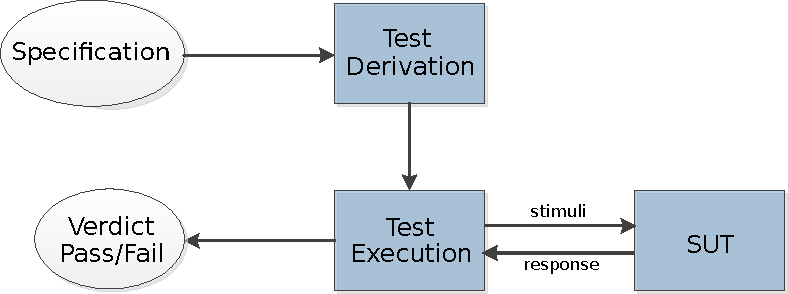
\includegraphics[width=0.75\textwidth]{model-based-testing.pdf}
  \end{center}
  \caption{A general model-based testing setup}
  \label{fig:model_based_testing}
\end{figure}

This type of model-based testing is called \textit{batch testing} or \textit{offline testing}. Another type of model-based testing is \textit{on the fly} testing. The main difference is that no test cases are derived, instead a transition in the model is chosen and tested on the system directly. The general architecture for this process is shown in Figure~\ref{fig:model_based_testing_on_the_fly}. A tool for on-the-fly testing is TorX~\cite{Tretmans:TorX}, which integrates automatic test generation, test execution, and test analysis. A version of this tool written in Java under continuous development is JTorX~\cite{Belinfante:JTorX}.

\begin{figure}[h]
  \begin{center}
    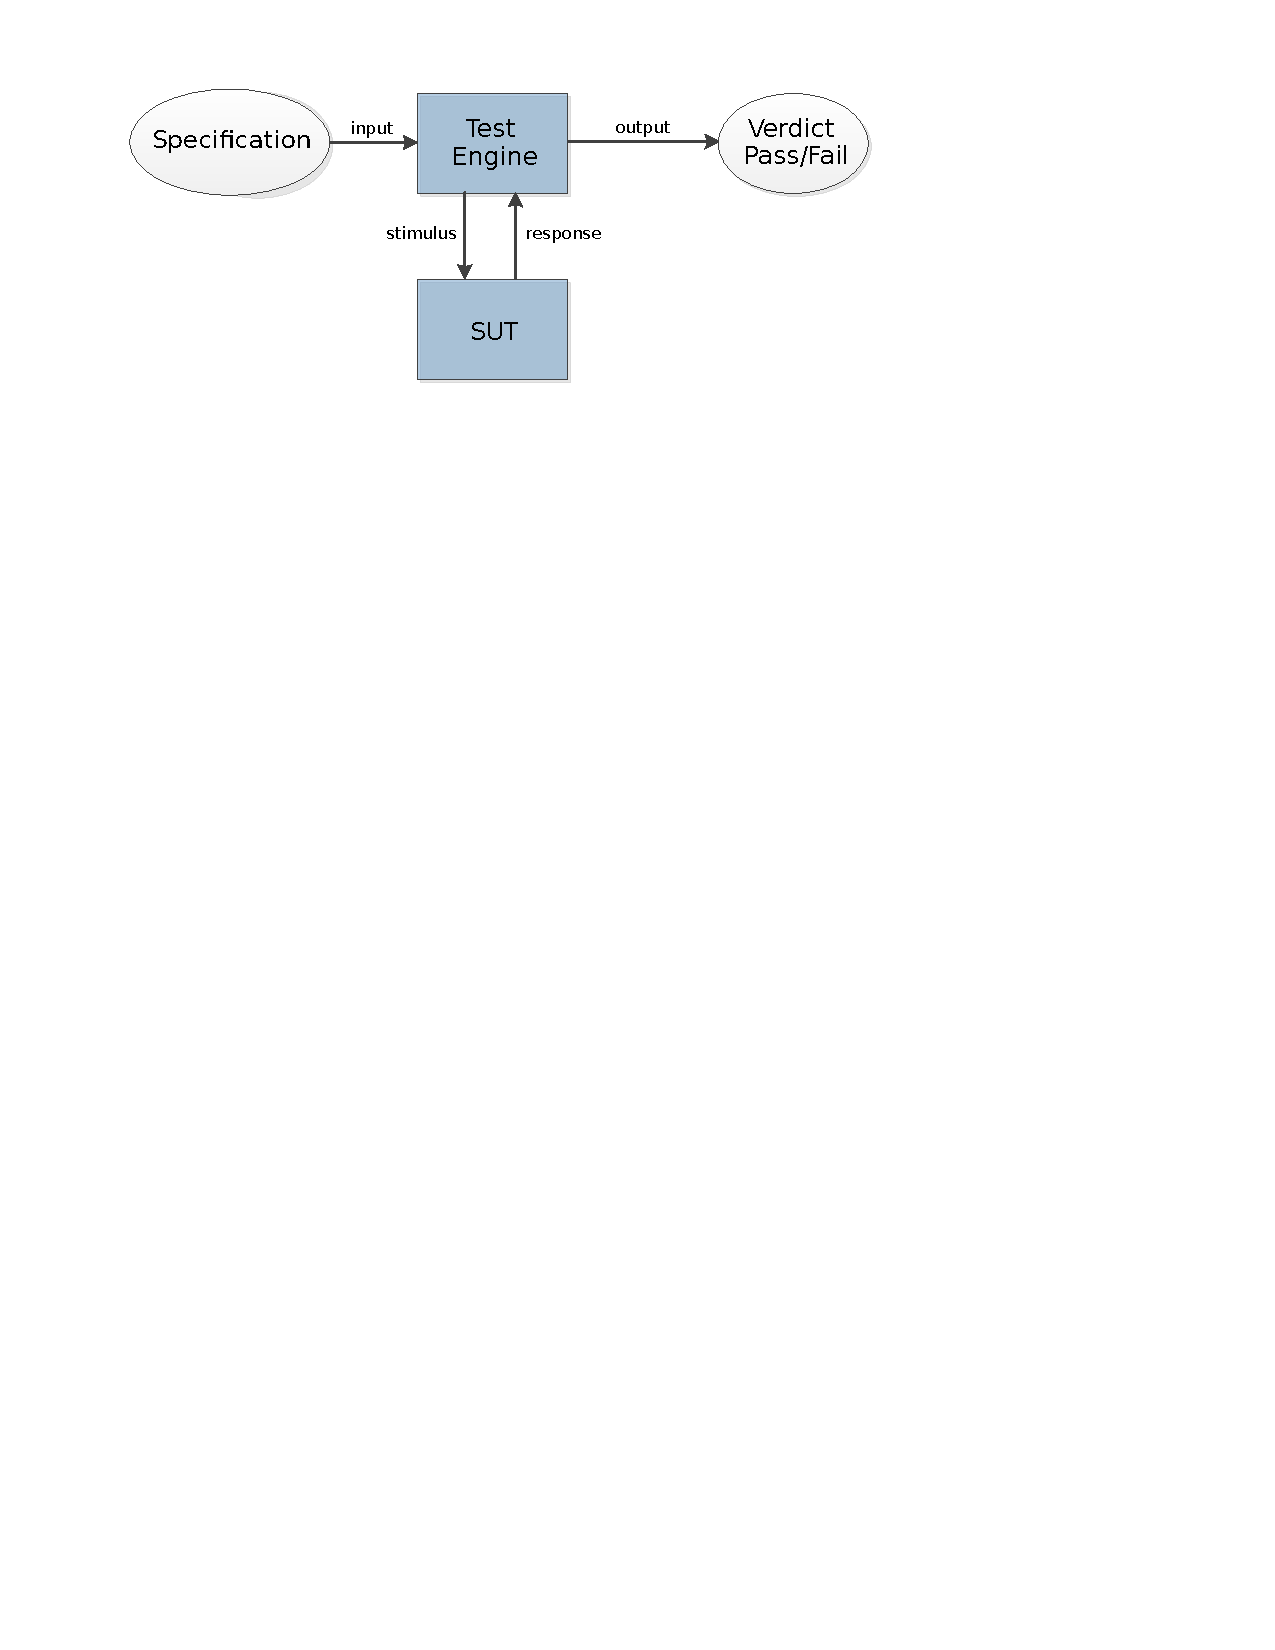
\includegraphics[width=0.75\textwidth]{mbt-on-the-fly.pdf}
  \end{center}
  \caption{A general 'on-the-fly' model-based testing setup}
  \label{fig:model_based_testing_on_the_fly}
\end{figure}

Variations of state machines and transition systems have been widely used as the underlying model for test generation. Other tools use the structure of data types to generate test data. First, two types of models are introduced. These are basic formalisms useful to understand the models in the rest of the paper. Then, the notion of \textit{coverage} is explained.

\subsection{Labelled Transition Systems}
A labelled transition system is a structure consisting of states with labelled transitions between them.

\begin{definition}
A labelled transition system is a 4-tuple	$\langle Q, L, T, q0\rangle$, where:
\begin{itemize}
\item $Q$ is a finite, non-empty set of states
\item $L$ is a finite set of labels
\item $T \in Q \times (L \cup \{\tau\}) \times Q$, with $\tau \notin L$, is the transition relation
\item $q0 \in Q$ is the initial state.
\end{itemize}
We write $q \xrightarrow{\mu}q'$ if there is a transition labelled $\mu$ from state q to state q', i.e., $(q, \mu, q') \in T$. The informal idea of such a transition is that when the system is in state $q$ it may perform action $\mu$, and go to state $q'$. 
\end{definition}

%Suppose that in state $q'$ the system can perform action $μ'$, i.e., $q'\xrightarrow{$\mu'$}q''$, then these transitions can be composed: q μ −q μ −−→q, which is written as q μ·μ −−−→q. In general, the
%composition of transitions q1
%μ1·μ2·...·μn −−−−−−−−→q2 expresses that the system, when in
%state q1, can perform the sequence of actions μ1·μ2· . . . ·μn, and may end in state
%q2. The use of may is important here: because of non-determinism, it may be
%the case that the system can also perform the same sequence of actions, but end
%in another state: q1
%μ1·μ2·...·μn −−−−−−−−→q3 with q2 = q3.

\subsection{Input-Output Transition Systems}
A useful type of transition system for model-based testing is the Input-Output Transition System (IOTS) by Tretmans~\cite{Tretmans:testgeneration}. Assuming that implementations communicate with their environment via inputs and outputs, this formalism is useful for describing system behavior. IOTSs have the same definition as LTSs with one addition: each label $l \in L$ has a type $t \in T$, where $T = \{input, output\}$. Each label can therefore specify whether the action represented by the label is a possible input or an expected output of the system under test.

An example of such an IOTS is shown in Figure~\ref{fig:iots_example}. This system allows an input of 20 or 50 cents and then outputs tea or coffee accordingly. The inputs are preceded by a question mark, the outputs are preceded by an exclamation mark. This system is a specification of a coffee machine. A test case can also be described by an IOTS with special pass and fail states. A test case for the coffee machine is given in Figure~\ref{fig:iots_test}. The test case shows that when an input of '50c' is done, an output of 'coffee' is expected from the tested system, as this results in a 'pass' verdict. When the system responds with 'tea', the test case results in a 'fail' verdict. The pass and fail verdicts are two special states in the test case, which are sink states, i.e., once in either of those the test case cannot leave that state. 

Test cases should always reach a pass or fail state within finite time. This requirement ensures that the testing process halts.
\begin{figure}[h]
  \begin{center}
    \subfloat[An IOTS]{\label{fig:iots_example}$\xymatrix{
    \bullet \ar[r]^{?50c} \ar[d]_{?20c} & \bullet \ar[d]^{\mathit{!coffee}} \\
    \bullet \ar[r]_{!tea}       & \bullet }$
}
    \subfloat[An IOTS test case]{\label{fig:iots_test}$\xymatrix{
    \bullet \ar[r]^{!50c} & \bullet \ar[r]^{\mathit{?coffee}} \ar[d]_{?tea} & {pass}\\
    & {fail}}$}
  \end{center}
  \caption{The specification of a coffee machine and a test case as an IOTS}
\end{figure}

%Unnecessary nondeterminism should be avoided in test cases \cite{Tretmans:ModelBasedTesting}: "In the first place, this implies that the test case itself is deterministic. In the second place, this means that a tester should never offer more than one input action (from the perspective of the implementation) at a time. Since the implementation is able to accept any input action, offering more inputs would always lead to an unnecessarily non-deterministic continuation of the test run. Having a deterministic test case does not imply that a test run has a unique result: due to non-determinism in the implementation under test, and due to non-determinism in the test run itself, the repetition of a test run may lead to a different result".

\subsection{Coverage}\label{sec:coverage}
The number of tests that can be generated from a model is potentially infinite. Therefore, there must be a test selection strategy to maximize the quality of the tests while minimizing the time spent testing. Coverage statistics help with test selection. Such statistics indicate how much of the SUT is tested. When the SUT is a black-box, typical coverage metrics are state and transition coverage of the model~\cite{Lee:testing, Nachmanson:testing, Hasan:testing}.

As an example, let us calculate the coverage metrics of the IOTS test case example in~\ref{fig:iots_test}. The test case tests one path through the specification and passes through 3 out of 4 states and 2 out of 4 transitions. The state coverage is therefore 75\% and the transition coverage is 50\%.

Coverage statistics are a useful metric for communicating how much of a system is tested.\marginpar{zoek referentie hiervoor}


	%\section{Symbolic Transition Systems}\label{sec:symbolic}
\textit{Symbolic Transition Systems} (STSs) combine a state oriented and data type oriented approach. These systems are used in practice in ATM and will therefore be part of GRATiS. In this section, previous work on STSs is given. The definitions of STSs and IOSTSs follow. An example of an IOSTS is then given. Next, the transformation of an STS to an LTS is explained and illustrated by an example. This transformation is useful when comparing STSs to systems that are not STSs. Finally, different coverage metrics on STSs are explained.

\subsection{Previous work}
STSs are introduced by Frantzen et al.~\cite{Frantzen:Symbolic}. This paper includes a detailed definition, on which the definition in section~\ref{sec:sts_definition} is based. The authors also give a sound and complete test derivation algorithm from specifications expressed as STSs. Deriving tests from a symbolic specification or \textit{Symbolic test generation} is introduced by Rusu et al.~\cite{rusu:symbolic}. Here, the authors use \textit{Input-Output Symbolic Transition Systems} (IOSTSs). These systems are very similar to the STSs in~\cite{Frantzen:Symbolic}. However, the definition of IOSTSs we will use in this report is based on the STSs by~\cite{Frantzen:Symbolic}. A tool that generates tests based on symbolic specifications is the STG tool, described in Clarke et al.~\cite{clarke:STG}.

\subsection{Definition}\label{sec:sts_definition}
An STS has \textit{locations} and \textit{switch relations}. If the STS represents a model of a software system, a location in the STS represents a state of the system, not including data values. A switch relation defines the transition from one location to another. The \textit{location variables} are a representation of the data values in the system. A switch relation has a \textit{gate}, which is a label representating the execution steps of the system. Gates have \textit{interaction variables}, which represent some input or output data value. Switch relations also have \textit{guards} and \textit{update mappings}. A guard is a term $\term \in \BooleanTerms(\Variables)$. The guard disallows using the switch relation when the valuation of the term results in $\mathit{false}$. When the valuation results in $\mathit{true}$, the switch relation of the guard is \textit{enabled}. An update mapping is a term-mapping of location variables. After the system switches to a new location, the variables in the update mapping will have the value corresponding to the valuation of the term.
\vspace{5px}
\begin{definition}
A Symbolic Transition System is a tuple $\langle \Locations,\initialLocation,\LocationVariables,\initializationFunction,\InteractionVariables,\Gates,\Switches\rangle$, where:
\begin{itemize}
\item $\Locations$\newnot{symbol:Locations} is a finite set of locations and $\initialLocation \in \Locations$\newnot{symbol:initialLocation} is the initial location.
\item $\LocationVariables \subseteq \Variables$\newnot{symbol:LocationVariables} is a finite set of location variables.
\item $\initializationFunction$\newnot{symbol:initializationFunction} is a term-mapping $\LocationVariables \rightarrow \Terms(\emptyset)$, representing the initialisation of the location variables.
\item $\InteractionVariables \subseteq \Variables$\newnot{symbol:InteractionVariables} is a set of interaction variables, disjoint from $\LocationVariables$.
\item $\Gates$\newnot{symbol:Gates} is a finite set of gates. The unobservable gate is denoted $\tau (\tau \notin \Gates)$; we write $\Gates_\tau$ for $\Gates \cup \{\tau\}$. The arity of a gate $\Gates\in\Gates_\tau$, denoted $arity(\Gates)$, is a natural number. The parameters of a gate $\Gates\in\Gates_\tau$, denoted $param(\Gates)$, are a tuple of length $arity(\Gates)$ of distinct interaction variables. We fix arity($\tau$) = 0, i.e. the unobservable gate has no interaction variables.
\item $\Switches \subseteq \Locations \times \Gates_\tau \times \BooleanTerms(\LocationVariables \cup \InteractionVariables) \times (\LocationVariables \rightarrow \Terms(\LocationVariables \cup \InteractionVariables)) \times \Locations$\newnot{symbol:Switches}, is the switch relation. We write $\location\xrightarrow{\Gates,\guard,\updateMapping}\location'$ instead of $(\location,\Gates,\guard,\updateMapping,\location')\in\Switches$, where $\guard$\newnot{symbol:guard} is referred to as the guard and $\updateMapping$\newnot{symbol:updateMapping} as the update mapping. We require $var(\guard) \cup var(\updateMapping \subseteq \LocationVariables \cup param(\Gates)$. We define $out(\location) \subset \Switches$ to be the outgoing switch relations from location $\location$.
\end{itemize}
\end{definition}

\subsection{Input-Output Symbolic Transition Systems}
An IOSTS can now easily be defined. The same difference between LTSs and IOTSs applies, namely each gate in an IOSTS has a type $\iotype \in \IOTypes$, where $\IOTypes = \{input, output\}$. As with IOSTSs, each gate is preceded by a '?' or '!' to indicate whether it is an input or an output respectively.

\subsection{Example}\label{sec:sts_example}
In Figure~\ref{fig:example_sts} the IOSTS of a simple board game is shown, where two players consecutively throw a die and move along four squares. The 'init' switch relation is a graphical representation of the variable initialization $\initializationFunction$. The values in the tuple of the IOSTS are defined as follows:

$\begin{array}{lcl}
\Locations & = & \{t, m\} \\
\initialLocation & = & t \\
\LocationVariables & = & \{T, P1, P2, D\} \\
\initializationFunction & = & \{T \mapsto 0, P1 \mapsto 0, P2 \mapsto 2, D \mapsto 0\} \\
\InteractionVariables & = & \{d, p, l\} \\
\Gates & = & \{?throw, !move\} \\
\Switches & = & \{t\xrightarrow{?throw, 1 <= d <= 6, D \mapsto d}m, \\
 & & m\xrightarrow{!move, T=1 \land l=(P1+D)\%4, P1 \mapsto l, T \mapsto 2}t, \\
 & & m\xrightarrow{!move, T=2 \land l=(P2+D)\%4, P2 \mapsto l, T \mapsto 1}t\}
\end{array}$

The variables $T, P1, P2$ and $D$ are the location variables symbolizing the player's turn, the positions of the players and the number of the die thrown respectively. The output gate $!move$ has $param = \langle p, l\rangle$ symbolizing which player moves to which location. The input gate $?throw$ has $param = \langle d\rangle$ symbolizing which number is thrown by the die. The switch relation with gate $?throw$ has the restriction that the number of the die thrown is between one and six and the update sets the location variable $D$ to the value of interaction variable $d$. The switch relations with gate $!move$ have the restriction that it must be the turn of the player moving and that the new location of the player is the number of steps ahead as thrown by the die. The update mapping sets the location of the player to the correct value and passes the turn to the next player. In Figure~\ref{fig:example_sts} the gates, guards and updates are separated by pipe symbols '|' respectively.

\begin{figure}[ht]
  \begin{center}
    $\xymatrix{
   \ar[rrrrr]^{init\:|\:true\:|\:T\mapsto 1,\:P1\mapsto 0,\:P2\mapsto 2,\:D\mapsto 0} &&&&& {t} \ar[rrrrrrrr]^{?throws(d:N)\,|\,1\,<=\,d\,<=\,6\,|\,D\mapsto d} &&&&&&&& {m} \ar@/_2pc/[llllllll]_{!move(p:N,l:N)\: |\: T=1 \:\land\: p=1 \:\land\: l = (P1+D)\%4\:|\:P1\mapsto l,\:T\mapsto 2} \ar@/^2pc/[llllllll]^{!move(p:N,l:N) \:|\: T=2 \:\land\: p=2 \land l = (P2+D)\,\%4\:|\: P2\mapsto l,\:T\mapsto 1}
}$

  \end{center}
  \caption{The STS of a board game example}
  \label{fig:example_sts}
\end{figure}

\subsection{STS to LTS mapping}\label{sec:sts_lts_trafo}
Consider an STS $J$ and an LTS $K$. There exists a mapping from the location and location variable valuations to the states of $K$ and from the switch relations and variable valuations of $J$ to the transitions of $K$, such that $K$ is an expansion of $J$. These relations are defined as follows:
$\begin{array}{ll}
\StsExpansionMapping_\States: & (\Locations \times (\LocationVariables \rightarrow \mathbb{U})) \rightarrow \States \\
\StsExpansionMapping_\Labels: & (\Gates \times (\InteractionVariables \rightarrow \mathbb{U})) \rightarrow \Labels \\
\StsExpansionMapping_\Transitions: & (\location\xrightarrow{\gate,\guard,\updateMapping}\location', \valuation: ((\LocationVariables \cup \InteractionVariables) \rightarrow \mathbb{U})) \mapsto (\StsExpansionMapping_\States(\location, \valuation \restriction \LocationVariables) \xrightarrow{\StsExpansionMapping_\Labels(\gate, \valuation \restriction\InteractionVariables)} \StsExpansionMapping_\States(\location', \valuation_{after}(\updateMapping)))
\end{array}$

\begin{comment}
These relations are constructed as follows: for a switch relation $r$ from location $A$ to location $B$, a valuation of the location variables $\nu_l$ and interaction variables $\nu_i$, $\mu_l:(A,\nu_l)$ maps to a state $q$, where $q$ is the source state of a transition $t$, if the result of the valuation $\nu:(\phi$ of $r, \nu_l \cup \nu_i)$ is true. $\nu_{l_new}$ is the new valuation of the location variables constructed by the valuation of $\rho$ of $r$. Then, the target state $q'$ of $t$ is the state mapped by $\mu_l:(B,\nu_{l_new}$). The label of $t$ is a textual representation of $\Gates$ of $r$ and $\nu_i$. Applying this rule for the topology to all locations, switch relations and concrete values for the variables, results in $L$. The start state $q0$ of $L$ is the state mapped by $\mu_l:(l_0,\initializationFunction)$. All states not reachable from $q0$ are removed from $L$.
\end{comment}

When the number of possible valuations for $\LocationVariables$ and $\InteractionVariables$ and the number of locations in an STS is considered to be finite, the transformation is always possible to an LTS with finite number of states.

An example of this transformation is shown in Figure~\ref{fig:example_trafo}. The label 'do(1)' in the LTS is a textual representation of the gate 'do' plus a valuation of the interaction variable 'd'. The transformation of a switch relation and concrete values to a transition is also called \textit{instantiating} the switch relation. Another term we will use for a switch relation with a set of concrete data values is an \textit{instantiated switch relation}.

\begin{figure}[ht]
  \begin{center}
    \subfloat[The STS]{\label{fig:trafo_sts}$\xymatrix{
   \ar[d]^{init\,|\,true\,|\,N\,:=\,0;} \\
   \bullet \ar@/^/[d]^{do(d:N)\,|\,1\,<=\,n\,<=\,2\,|\,N\,:=\,n} \\
   \bullet \ar@/^/[u]^{sub(i:N)\,|\,1\,<=\,i\,<=\,2\,|\,N\,:=\,N\,-\,i}}$
}\hspace{20px}
    \subfloat[The LTS]{\label{fig:trafo_lts}$\xymatrix{
\fbox{$\location_0, N=2$} & \ar[r] & \fbox{$\location_0, N=0$} \ar@/^/[ddll]^{do(1)} \ar@/^/[ddrr]^{do(2)} && \\ \\
 \fbox{$\location_1, N=1$} \ar@/^/[uurr]^{sub(1)} \ar@/^/[ddrr]^{sub(2)} && \fbox{$\location_0, N=1$} \ar[ll]^{do(1)} \ar@/^/[rr]^{do(2)} && \fbox{$\location_1, N=2$} \ar@/^/[ll]^{sub(1)} \ar@/^/[uull]^{sub(2)} \\\\
 && \fbox{$\location_0, N=-1$} \ar@/^/[uull]^{do(1)} \ar[uurr]^{do(2)}}$
}
  \end{center}
  \caption{An example of a transformation of an STS to an LTS}
  \label{fig:example_trafo}
\end{figure}

\subsection{Coverage}\label{sec:sts_coverage}
The simplest metric to describe the coverage of an STS is the location and switch-relation coverage, which express the percentage of locations and switch relations tested in the test run. Measuring state and transition coverage of an STS is possible using the LTS resulting from the STS transformation. However, this metric is not always useful, because the number of states and transitions in the LTS depend on the number of unique combinations of concrete values of the variables in the STS. This is potentially very large. For example, when the guards of the switch relations in Figure~\ref{fig:trafo_sts} are removed, the transformation leads to an LTS with a state and transition for each possible value of an integer. It is often infeasable to test every data value in the STS. The most interesting data values to test can be found by \textit{boundary-value analysis} and \textit{equivalence partitioning}. For an explanation of these terms we refer to~\cite{Myers:2004}.\marginpar{A:Explain! (example) V: Ik denk eigenlijk niet dat deze technieken relevant gaan zijn uiteindelijk} Boundary-value analysis was found to be most effective by Reid~\cite{Reid:partitioning} in fault detection.

\textit{Data coverage} expresses the percentage of data tested in the test run, considering data to be similar if located in the same partition and a better representative of the partition if located close to the partition boundary. These properties of the tested data affect the data coverage percentage.

	%\section{Graph Transformation}\label{sec:graph}
A \textit{graph grammar} is composed of a start graph and a set of transformation rules. The start graph describes the system in its initial state. The transformation rules describe what changes are made to the graph, resulting in a new graph which describes the system in its new state. The definition is as follows.

\begin{definition}
A graph grammar is a tuple $\langle G, R\rangle$, where:
\begin{itemize}
  \item $G$ is the start graph
  \item $R$ is a set of graph transformation rules
\end{itemize}
\end{definition} 

The rest of this section is ordered as follows: first, graphs and graph morphisms are explained. This is then used to explain graph transformation rules, followed by the definition of a graph grammar. Then, the definition of a \textit{Graph Transition System} (GTS) is given. An example of a graph grammar and a GTS is then given. Finally, a method for transforming a GTS to an STS is given. For a more detailed overview of graph grammars, we refer to~\cite{Rensink:graph_grammars, Heckel2006187, Andries1999}.

\subsection{Graphs \& morphisms}
\begin{definition}
A graph is a tuple $\langle L, N, E\rangle$, where:
\begin{itemize}
  \item $L$ is a set of labels
  \item $N$ is a set of nodes, where each $n \in N$ has a label $l \in L$
  \item $E$ is a set of edges, where each $e \in E$ has a label $l \in L$ and nodes $source,target \in N$
\end{itemize}
\end{definition}

A graph $H$ has an \textit{occurrence} in a graph $G$, denoted by $H \rightarrow G$, if there is a mapping from the nodes and the edges of $H$ to the nodes and the edges of $G$ respectively. Such a mapping is called a \textit{morphism}. An element $e$ in graph $H$ is then said to have an \textit{image} in graph $G$ and $e$ is a \textit{pre-image} of the image. A graph $H$ has a partial morphism to a graph $G$ if there are elements in $H$ without an image in $G$.

\subsection{Graph transformation rules}
\begin{definition}
A transformation rule is a tuple $\langle \mathit{LHS}, \mathit{NAC}, \mathit{RHS}, \mathit{M}\rangle$, where:
\begin{itemize}
  \item $\mathit{LHS}$ is a graph representing the left-hand side of the rule
  \item $\mathit{NAC}$ is a set of graphs representing the negative application conditions
  \item $\mathit{RHS}$ is a graph representing the right-hand side of the rule
  \item $\mathit{M_{RHS}}$ is a partial morphism of $\mathit{LHS}$ to $\mathit{RHS}$ 
  \item $\mathit{M_{NAC}}$ are partial morphisms of $\mathit{LHS}$ to each $n \in \mathit{NAC}$
\end{itemize}
\end{definition}

A rule $R$ is applicable on a graph $G$ if its $\mathit{LHS}$ has an occurrence in $G$ and $\not\ exists n \in \mathit{NAC}$ such that $n$ has an occurence in $G$ and $\forall e \in \mathit{LHS}$, if $e$ has an image $i$ in $n$ and an image $j$ in $G$, then $j$ should be an image of $j$. After the rule application, all elements in $\mathit{LHS}$ not part of $\mathit{M_{RHS}}$, i.e. they do not have an image in $\mathit{RHS}$, are removed from $G$ and all elements in $\mathit{RHS}$ not part of $\mathit{M_{RHS}}$, i.e. they do not have a pre-image in $\mathit{LHS}$, are added to $G$.

\subsection{Graph Transition Systems}
By repeatedly applying graph transformation rules to the start graph and all its consecutive graphs, a graph grammar can be explored to reveal a \textit{Graph Transition System} (GTS). This transition system consists of \textit{graph states} connected by \textit{rule transitions}.

\begin{definition}
A graph transition system is an 8-tuple	$\langle S, L, T, G, R, M_G, M_R, s0\rangle$, where:
\begin{itemize}
\item $S$ is a finite, non-empty set of graph states
\item $L$ is a finite set of labels. For each label $l\in L$, the arity of $l$, denoted $\mathit{arity(l)}$, is a natural number. The parameters of $l$, denoted $\mathit{param(l)}$, is a tuple of length $\mathit{arity(l)}$ of variables.
\item $T \in S \times (L \cup \{\tau\}) \times S$, with $\tau \notin L$, is the rule transition relation. The parameters of a transition $t \in T$ with label $l \in L$, denoted $\mathit{param(t)}$, is a tuple of length $\mathit{arity(l)}$ of constants, such that $\Sigma:\mathit{param(l)} \mapsto \mathit{param(t)}$ is the valuation of the variables of the label.
\item $G$ is a set of graphs.
\item $R$ is a set of rules.
\item $M_G$ is a mapping $\forall s \in S . s \mapsto g \in G \land \not\exists s' \in S . s \neq s' \land s' \mapsto g \in M_G$
\item $M_R$ is a mapping $\forall t \in T . t \mapsto r \in R \land \not\exists t' \in T . t \neq t' \land t' \mapsto r \in M_R$
\item $s0 \in s$ is the initial graph state.
\end{itemize}
We write $s \xrightarrow{\mu}s'$ if there is a rule transition labelled $\mu$ from state s to state s', i.e., $(s, \mu, s') \in T$.
\end{definition}

These systems are very similar to LTSs. A GTS can be transformed to an LTS by omitting the graphs, rules, mappings and parameters on labels.

\subsection{Example}\label{sec:gts_example}
Figure \ref{fig:gts} shows an example of the start graph and one rule of a graph grammar. $\mathit{M_{RHS}}$ maps the $A$ and $B$ nodes in $\mathit{LHS}$ to the A and B nodes in $\mathit{RHS}$ respectively. $\mathit{M_{NAC}}$ maps the $A$ node in $\mathit{LHS}$ to the $A$ node in both graphs in $\mathit{NAC}$. The a-edge in $\mathit{LHS}$ is mapped to the a-edge in the first $\mathit{NAC}$. The $\mathit{LHS}$ of the rule has an occurrence in the start graph, as the $A$ and $B$ nodes connected by the a-edge exist in both graphs. None of the graphs in the $\mathit{NAC}$ have an occurrence in the start graph, because the $C$ node does not exist in the start graph. The new graph after applying the rule is in Figure~\ref{fig:gg_result}.

\begin{figure}[ht]
  \begin{center}
    \subfloat[The start graph]{\label{fig:gg_graph}$\xymatrix{
   \fbox{A} \ar[r]^{a} & \fbox{B}
}$
}\hspace{20px}
    \subfloat[The LHS]{\label{fig:gg_lhs}$\xymatrix{
   \fbox{A} \ar[r]^{a} & \fbox{B}
}$
}\hspace{20px}
    \subfloat[The first NAC]{\label{fig:gg_nac1}$\xymatrix{
   \fbox{A} \ar[r]^{a} & \fbox{C}
}$
}\hspace{20px}
    
    \subfloat[The second NAC]{\label{fig:gg_nac2}$\xymatrix{
   \bullet \ar@(dl,dr)[]_{A} \ar[r]^{b} & \bullet \ar@(dl,dr)[]_{C}
}$
}\hspace{20px}
    \subfloat[The RHS]{\label{fig:gg_rhs}$\xymatrix{
   \bullet \ar@(dl,dr)[]_{A} \ar[r]^{b} & \bullet \ar@(dl,dr)[]_{B}
}$
}\hspace{20px}
    \subfloat[The result]{\label{fig:gg_result}$\xymatrix{
   \bullet \ar@(dl,dr)[]_{A} \ar[r]^{b} & \bullet \ar@(dl,dr)[]_{B}
}$
}
  \end{center}
  \caption{An example of a graph grammar}
  \label{fig:gts}
\end{figure}

\subsection{GTS to STS transformation}\label{sec:gts_sts_trafo}
The method described here transforms a GTS to an STS. This STS is not \textit{optimal}, i.e. it is reducible to an STS with fewer locations and switch relations. This method only serves as a proof used in section~\ref{sec:init_design}.

For each graph state $s \in S$ create a location $l \in L$. The start location $l_0 \in L$ is the location created by the state $s0 \in S$. Set $\mathcal{V} = \emptyset$ and $\imath = \emptyset$. For each label $l \in L$ create a gate $\lambda \in \Lambda$. For each $p \in \mathit{param}(l)$ create an interaction variable $i \in \mathcal{I}$ of the same type as $p$ and add $i$ to $param(\lambda)$. Set $\mathit{arity}(\lambda) = \mathit{arity}(l)$. For each rule transition $t \in T$ create a switch relation $r \in \rightarrow$, where:
\begin{itemize}
  \item the source and the target locations of $r$ are the locations created by the source and target graph states of the rule transition.
  \item the gate of $r$ is the gate created by the label on the transition.
  \item for each $p \in \mathit{param}(l)$ and $i \in \mathcal{I}$ created by $p$ create an $i = p$ expression. The guard of $r$ is those expressions joined by the $\land$ operator.
  \item the update mapping of $r$ is empty.
\end{itemize}

An example of such a transformation is done using the LTS in Figure~\ref{fig:trafo_lts}. Consider this LTS to be a GTS where the states are graph states, the transitions are rule transitions with label 'do' with $\mathit{arity(do)} = 1$ and $\mathit{param(do)}$ the integers between brackets are The STS resulting from the transformation is in Figure~\ref{fig:trafo_basic_sts}.

\begin{figure}[ht]
  \begin{center}
    $\xymatrix{
   \bullet \ar[rr]^{do(n:N) | n = 1 | } \ar[dd]_{do(n:N) | n = 2 | } && \bullet \ar@(ul,ur)^{do(n:N) | n = 1 | } \ar@(d,r)[ddll]^{do(n:N) | n = 2 | } \\ \\
   \bullet \ar@/^/[uurr]|-{do(n:N) | n = 1 | } \ar@(dl,dr)[]_{do(n:N) | n = 2 | }}$
  \end{center}
  \caption{The basic STS resulting from the transformation of the LTS in Figure~\ref{fig:trafo_lts}}
  \label{fig:trafo_basic_sts}
\end{figure}

	%\section{Tooling}\label{sec:tooling}

\subsection{ATM}\label{sec:descriptionaxini}
ATM is a web-based application, developed in the Ruby on Rails framework. It is used to test the software of several big companies in the Netherlands since 2006. It is under continuous development by Axini.

The architecture is shown graphically in Figure~\ref{fig:axini_tool}. It has a similar structure to the on-the-fly model-based testing tool architecture in Figure~\ref{fig:model_based_testing_on_the_fly}.

\begin{figure}[h!]
  \begin{center}
    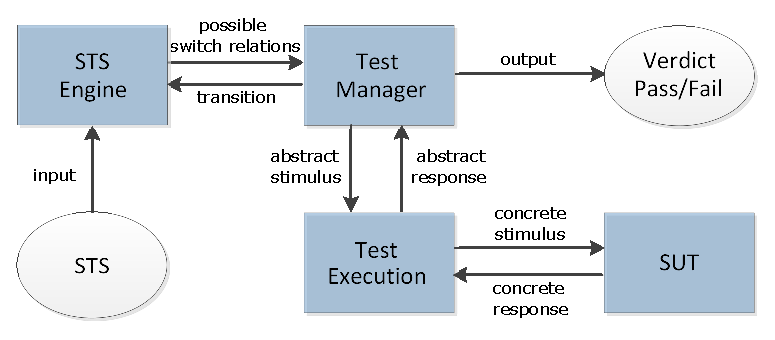
\includegraphics[width=0.75\textwidth]{axini_tool.eps}
  \end{center}
  \caption{Architecture of ATM}
  \label{fig:axini_tool}
\end{figure}

The tool functions as follows: 
\begin{enumerate}
  \item An STS is given to an STS Engine, which passes the possible switch relations from the current state to the Test Manager.
  \item The Test Manager chooses a switch relation and the data values, based on a test strategy. In the LTS in the STS-to-LTS transformation, this choice is represented by one transition. 
  \item The label of the transition is given to the Test Execution component as an \textit{abstract stimulus}. The term abstract is used here to indicate that the transition is specific to the model. It represents some computation steps taken in the SUT. For instance, a transition with label 'connect?' is an abstract stimulus of the actual setup of a TCP connection between two distributed components of the SUT. 
  \item The translation of an abstract stimulus to a concrete stimulus is done by the Test Execution component. This component provides the stimulus to the SUT. When the SUT responds, the Test Execution component translates this response to an abstract response. For instance, the Test Execution component receives an HTTP response that the TCP connect was succesful. This is a concrete response, which the Test Execution component translates to an abstract response, such as a transition with label 'ok!'. The Test Manager is notified with this abstract response.
  \item The Test Manager updates the STS Engine on which transition was chosen as stimulus and which transition was detected based on the response of the SUT. If this latter transition is possible according to the model, the Test Manager gives a pass verdict for this test. Otherwise, the result is a fail verdict.
\end{enumerate}

\subsection{GROOVE}\label{sec:descriptiongroove}
GROOVE is an open source, graph-based modelling tool in development at the University of Twente since 2004. It has been applied to several case studies, such as model transformations and security and leader election protocols~\cite{Ghamarian:GROOVE}.

The architecture of the GROOVE tool is shown graphically in Figure~\ref{fig:groove_tool}. A GTS is given as input to a Rule Applier component, which determines the possible rule transitions. An Exploration Strategy can be started or the user can explore the states manually using the GUI. These components request the possible rule transitions and respond with the chosen rule transition (based on the exploration strategy or the user input). The Exploration Strategy can do an exhaustive search, resulting in a GTiS. The graph states and rule transitions in this GTiS can then be inspected using the GUI.

\begin{figure}[h]
  \begin{center}
    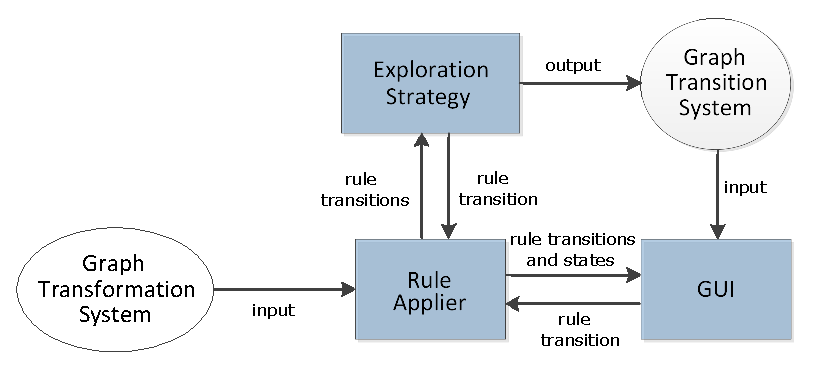
\includegraphics[width=0.75\textwidth]{groove_tool.eps}
  \end{center}
  \caption{The GROOVE Tool}
  \label{fig:groove_tool}
\end{figure}

%GROOVE provides parameters for the labels on the transitions in a GTiS by indicating which node(s) in a rule should be the parameter(s). 
\subsection{Comparison of the examples}\label{sec:comparison}
The models of the boardgame example in Figures~\ref{fig:example_sts} and \ref{fig:example_groove} are very different. In this section the STS and the GTS of the example are compared.

\subsubsection{Comparison of behavior}
The GTS of the boardgame example has a number of consecutive transitions when a player moves. The $move$ rule puts the \textbf{Player} on the next \textbf{Location} and lowers the remaining 'moves' by one. This is different from the STS, which updates the location variable in one transition. The effect is that the behavior of both systems is different; one specifies the movement of a \textbf{Player} as: "Player p moves to Location l", the other as: "The Player with the turn moves to the next Location". Which behavior is required when this boardgame would be tested depends on the implementation of the game. However, to show the power of the GTS formalism, Figure~\ref{fig:example_groove2} shows the GTS with the same behavior as the STS. It models the location as a variable and updates this variable in one transition. It also identifies the \textbf{Players} by giving them a number.

\begin{figure}[h]
  \begin{center}
    \subfloat[The start graph]{\label{fig:example_groove_start2}% To use this figure in your LaTeX document
% import the package groove/resources/groove2tikz.sty
%
% Special colors
\begin{tikzpicture}[
% Special color styles
scale=\tikzscale]
\node[node] (n9)  at (1.975, -0.725) {\ml{\textbf{Location}\\field = 1\\field = 3\\field = 2\\field = 0}};
\node[node] (n0)  at (0.825, -0.875) {\ml{\textbf{Die}\\canThrow = 1\\canThrow = 2\\canThrow = 3\\canThrow = 4\\canThrow = 5\\canThrow = 6}};
\node[node] (n11)  at (2.965, -0.660) {\ml{\textbf{Player}\\\textit{turn}\\at = 0\\number = 1}};
\node[node] (n12)  at (3.945, -0.595) {\ml{\textbf{Player}\\at = 2\\number = 2}};
\userdefinedmacro
\end{tikzpicture}
\renewcommand{\userdefinedmacro}{\relax}
}\quad
    \subfloat[The throw rule]{\label{fig:example_groove_throw2}% To use this figure in your LaTeX document
% import the package groove/resources/groove2tikz.sty
%
% Special colors
\begin{tikzpicture}[
% Special color styles
scale=\tikzscale]
\node[node] (n5)  at (1.595, -1.295) {\ml{\textbf{Die}}};
\node[nacnode, attr] (n2)  at (0.495, -1.325) {\ml{\textbf{int}}};
\node[node, attr] (n4)  at (1.605, -0.415) {\ml{\textbf{int}}};
\node[node] (n1)  at (0.545, -0.470) {\ml{\textbf{Player}\\\textit{turn}}};
\path[edge](n5.north -| 1.605, -0.415) -- node[lab]{canThrow} (n4) ;
\path[newedge](n1.east |- 1.605, -0.415) -- node[newlab]{throws} (n4) ;
\path[nacedge](n1.south -| 0.495, -1.325) -- node[naclab]{throws} (n2) ;
\userdefinedmacro
\end{tikzpicture}
\renewcommand{\userdefinedmacro}{\relax}
}
    \subfloat[The move rule]{\label{fig:example_groove_move2}% To use this figure in your LaTeX document
% import the package groove/resources/groove2tikz.sty
%
% Special colors
\begin{tikzpicture}[
% Special color styles
scale=\tikzscale]
\node[node, attr] (n1)  at (0.965, -1.520) {\ml{\textbf{int}}};
\node[node] (n0)  at (1.070, -0.680) {\ml{\textbf{Player}\\{\color{\blue}\textit{$-$ turn}}\\{\color{\green}at := (at $+$ throws) \% 4}}};
\node[node] (n2)  at (2.540, -0.660) {\ml{\textbf{Player}\\{\color{\green}\textit{$+$ turn}}}};
\path[deledge](n0.south -| 0.965, -1.520) -- node[dellab]{throws} (n1) ;
\path[edge, -](n2.west |- 1.070, -0.680) -- node[lab]{\textit{!=}} (n0) ;
\userdefinedmacro
\end{tikzpicture}
\renewcommand{\userdefinedmacro}{\relax}
}
  \end{center}
  \caption{Another GTS model of the board game example}
  \label{fig:example_groove2}
\end{figure}

The new GTS loses many advantages by structuring it in this way: the overview of the board is gone, the rules are less visual and extending the locations in different directions is much harder. On the other hand, there are less rules and the graphs are more compact. However, when finding the GTiS corresponding to this GTS, the labels of the transitions of that GTiS do not reflect the 'move(p:N, l:N)' label of the STS. This should be done by marking the correct nodes as described in section~\ref{sec:gts_example}. The problem is that the result of the equation in the 'move' rule is only derived when the rule is applied. Figure~\ref{fig:move3} shows a rule where the equation is shown graphically. The die roll, connected by the 'throws' edge, and the number of the \textbf{Location} the \textbf{Player} is at are added. The result is represented by the \textbf{int} node connected by the 'add' edge. This result modulo 4 is represented by the \textbf{int} node connected by the 'mod' edge. This node is marked as the second parameter, the number of the \textbf{Player} is marked as the first parameter. This labels the transitions with which player moves to which location.

\begin{figure}[h]
  \begin{center}
    % To use this figure in your LaTeX document
% import the package groove/resources/groove2tikz.sty
%
% Special colors
\begin{tikzpicture}[
% Special color styles
scale=\tikzscale]
\node[node] (n0)  at (1.985, -0.650) {\ml{\textbf{Player}\\{\color{\blue}\textit{$-$ turn}}}};
\node[node, attr] (n8)  at (2.405, -2.195) {\ml{\textbf{int}}};
\node[node, attr] (n5)  at (0.375, -0.655) {\ml{\textbf{int}}};
\node[parnode] (n5p)  at (n5.north west) {0};
\node[node, attr] (n4)  at (0.965, -1.485) {\ml{\textbf{int}}};
\node[node, prod] (n9)  at (3.445, -2.185) {\ml{\textit{$\pi$1 = 4}}};
\node[node] (n2)  at (3.455, -0.640) {\ml{\textbf{Player}\\{\color{\green}\textit{$+$ turn}}}};
\node[node, attr] (n10)  at (3.425, -1.395) {\ml{\textbf{int}}};
\node[parnode] (n10p)  at (n10.north west) {1};
\node[node, attr] (n7)  at (1.935, -1.475) {\ml{\textbf{int}}};
\node[node, prod] (n6)  at (1.395, -2.205){};
\path[edge] (n9)  -- node[lab]{mod} (n10) ;
\path[edge] (n6)  -- node[lab]{$\pi$0} (n4) ;
\path[edge](n0.west |- 0.375, -0.655) -- node[lab]{number} (n5) ;
\path[deledge](n0.south -| 1.935, -1.475) -- node[dellab]{at} (n7) ;
\path[deledge] (n0)  -- node[dellab]{throws} (n4) ;
\path[edge] (n9)  -- node[lab]{$\pi$0} (n8) ;
\path[edge, -](n2.west |- 1.985, -0.650) -- node[lab]{\textit{!=}} (n0) ;
\path[edge] (n6)  -- node[lab]{add} (n8) ;
\path[edge] (n6)  -- node[lab]{$\pi$1} (n7) ;
\path[newedge] (n0)  -- node[newlab]{at} (n10) ;
\userdefinedmacro
\end{tikzpicture}
\renewcommand{\userdefinedmacro}{\relax}

  \end{center}
  \caption{An alternative move rule}
  \label{fig:move3}
\end{figure}

\subsubsection{Comparison of Transition Systems}
The GTiS of a GTS can be found using GROOVE and the STS can be transformed to an LTS. The two GTSs and the STS of the board game example result in three transition systems which can be compared.

The GTS from Figure~\ref{fig:example_groove} generates a GTiS with 32 states with 52 transitions, which can be seen visually in Figure~ \ref{fig:statespace_groove1}. The GTS from Figure \ref{fig:example_groove2}, using the 'move' rule from Figure~\ref{fig:move3}, generates 224 states with 384 transitions, shown as GTiS in Figure~\ref{fig:statespace_groove2}. The reason of the difference in number of states and transitions is that the board is circular: to the first GTS, the players being at locations 1 and 3 is the same as them being at locations 2 and 4. However, this is not the same to the second GTS. Also, for the first GTS it does not matter which \textbf{Player} node is at a \textbf{Location} node; they are the same apart from which \textbf{Player} has the 'turn'. As an example, consider the start graph in Figure~\ref{fig:example_groove}. If both players throw a '1' and move to the next location, the state is as shown in Figure~\ref{fig:symmetry_example}. Both states are symmetrical and therefore they are the same state. This leads to a \textit{symmetry reduction} of the statespace for the first GTS.

\begin{figure}[h]
  \begin{center}
    % To use this figure in your LaTeX document
% import the package groove/resources/groove2tikz.sty
%
% Special colors
\begin{tikzpicture}[
% Special color styles
scale=\tikzscale]
\node[node] (n9)  at (4.245, -1.375) {\ml{\textbf{Location}}};
\node[node, bold] (n0)  at (1.585, -0.865) {\ml{\textbf{Die}\\canThrow = 1\\canThrow = 2\\canThrow = 3\\canThrow = 4\\canThrow = 5\\canThrow = 6}};
\node[node] (n7)  at (5.625, -1.935) {\ml{\textbf{Location}}};
\node[node, bold] (n11)  at (3.055, -0.520) {\ml{\textbf{Player}\\\textit{turn}}};
\node[node] (n12)  at (5.615, -0.525) {\ml{\textbf{Player}}};
\node[node] (n8)  at (2.995, -1.895) {\ml{\textbf{Location}}};
\node[node] (n10)  at (4.265, -2.455) {\ml{\textbf{Location}}};
\path[edge] (n10)  -- node[lab]{next} (n8) ;
\path[edge] (n7)  -- node[lab]{next} (n10) ;
\path[edge] (n9)  -- node[lab]{next} (n7) ;
\path[edge] (n11)  -- node[lab]{at} (n9) ;
\path[edge] (n8)  -- node[lab]{next} (n9) ;
\path[edge] (n12)  -- node[lab]{at} (n10) ;
\userdefinedmacro
\end{tikzpicture}
\renewcommand{\userdefinedmacro}{\relax}

  \end{center}
  \caption{An example of a state symmetrical with the state in Figure~\ref{fig:example_groove}}
  \label{fig:symmetry_example}
\end{figure}

The LTS where the STS in Figure~\ref{fig:example_sts} is transformed to has 224 states and 384 transitions. This is calculated by taking all possibilities of the data values except for the die roll. This leads to 32 states ($4 \times 4 \times 2$). These 32 'throw' states each have 6 'throw?' transitions to a 'move' state, thus there are 192 'move' states. The 'move' states only have one transition back to a 'throw' state. There are $6 \times 32 + 192 \times 1 = 384$ transitions.

\begin{figure}[h]
  \begin{center}
    \resizebox{\textwidth}{!}{% To use this figure in your LaTeX document
% import the package groove/resources/groove2tikz.sty
%
% Special colors
\begin{tikzpicture}[
% Special color styles
scale=\tikzscale]
\node[node, start] (s0)  at (4.240, -0.155) {\ml{\textit{s0}}};
\node[node] (s1)  at (0.590, -0.865) {\ml{\textit{s1}}};
\node[node] (s2)  at (1.870, -0.865) {\ml{\textit{s2}}};
\node[node] (s3)  at (5.130, -0.865) {\ml{\textit{s3}}};
\node[node] (s4)  at (6.050, -0.865) {\ml{\textit{s4}}};
\node[node] (s5)  at (6.970, -0.865) {\ml{\textit{s5}}};
\node[node] (s6)  at (7.890, -0.865) {\ml{\textit{s6}}};
\node[node] (s7)  at (0.590, -1.575) {\ml{\textit{s7}}};
\node[node] (s8)  at (1.870, -1.575) {\ml{\textit{s8}}};
\node[node] (s9)  at (5.130, -1.575) {\ml{\textit{s9}}};
\node[node] (s10)  at (6.055, -1.575) {\ml{\textit{s10}}};
\node[node] (s11)  at (6.975, -1.575) {\ml{\textit{s11}}};
\node[node] (s12)  at (7.895, -1.575) {\ml{\textit{s12}}};
\node[node] (s13)  at (0.595, -2.285) {\ml{\textit{s13}}};
\node[node] (s14)  at (1.875, -2.285) {\ml{\textit{s14}}};
\node[node] (s15)  at (5.135, -2.285) {\ml{\textit{s15}}};
\node[node] (s16)  at (6.055, -2.285) {\ml{\textit{s16}}};
\node[node] (s17)  at (6.975, -2.285) {\ml{\textit{s17}}};
\node[node] (s18)  at (7.895, -2.285) {\ml{\textit{s18}}};
\node[node] (s19)  at (0.595, -2.995) {\ml{\textit{s19}}};
\node[node] (s20)  at (1.875, -2.995) {\ml{\textit{s20}}};
\node[node] (s21)  at (2.665, -2.995) {\ml{\textit{s21}}};
\node[node] (s22)  at (3.915, -1.325) {\ml{\textit{s22}}};
\node[node] (s23)  at (4.625, -3.025) {\ml{\textit{s23}}};
\node[node] (s24)  at (5.635, -2.995) {\ml{\textit{s24}}};
\node[node] (s25)  at (6.625, -2.995) {\ml{\textit{s25}}};
\node[node] (s26)  at (5.145, -3.665) {\ml{\textit{s26}}};
\node[node] (s27)  at (0.595, -3.705) {\ml{\textit{s27}}};
\node[node] (s28)  at (1.865, -3.845) {\ml{\textit{s28}}};
\node[node] (s29)  at (2.855, -3.395) {\ml{\textit{s29}}};
\node[node] (s30)  at (3.435, -1.295) {\ml{\textit{s30}}};
\node[node] (s31)  at (0.595, -4.415) {\ml{\textit{s31}}};
\path[edge] (s0)  -- node[lab]{throws(3)} (s1) ;
\path[edge] (s0)  -- node[lab]{throws(2)} (s2) ;
\path[edge] (s0)  -- node[lab]{throws(1)} (s3) ;
\path[edge] (s0)  -- node[lab]{throws(5)} (s4) ;
\path[edge] (s0)  -- node[lab]{throws(6)} (s5) ;
\path[edge] (s0)  -- node[lab]{throws(4)} (s6) ;
\path[edge](s1.south -| 0.590, -1.575) -- node[lab]{move(1)} (s7) ;
\path[edge](s2.south -| 1.870, -1.575) -- node[lab]{move(1)} (s8) ;
\path[edge](s3.south -| 5.130, -1.575) -- node[lab]{move(1)} (s9) ;
\path[edge](s4.south -| 6.055, -1.575) -- node[lab]{move(1)} (s10) ;
\path[edge](s5.south -| 6.975, -1.575) -- node[lab]{move(1)} (s11) ;
\path[edge](s6.south -| 7.895, -1.575) -- node[lab]{move(1)} (s12) ;
\path[edge](s7.south -| 0.595, -2.285) -- node[lab]{move(1)} (s13) ;
\path[edge](s8.south -| 1.875, -2.285) -- node[lab]{move(1)} (s14) ;
\path[edge](s9.south -| 5.135, -2.285) -- node[lab]{nextTurn()} (s15) ;
\path[edge](s10.south -| 6.055, -2.285) -- node[lab]{move(1)} (s16) ;
\path[edge](s11.south -| 6.975, -2.285) -- node[lab]{move(1)} (s17) ;
\path[edge](s12.south -| 7.895, -2.285) -- node[lab]{move(1)} (s18) ;
\path[edge](s13.south -| 0.595, -2.995) -- node[lab]{move(1)} (s19) ;
\path[edge](s14.south -| 1.875, -2.995) -- node[lab]{nextTurn()} (s20) ;
\path[edge] (s15)  -- node[lab]{throws(3)} (s21) ;
\path[edge] (s15)  -- node[lab]{throws(2)} (s22) ;
\path[edge] (s15)  -- node[lab]{throws(1)} (s23) ;
\path[edge] (s15)  -- node[lab]{throws(5)} (s24) ;
\path[edge] (s15)  -- node[lab]{throws(6)} (s25) ;
\path[edge](s15.south -| 5.145, -3.665) -- node[lab]{throws(4)} (s26) ;
\path[edge] (s16)  -- node[lab]{move(1)} (s22) ;
\path[edge] (s17)  -- node[lab]{move(1)} (s21) ;
\path[edge] (s18)  -- node[lab]{move(1)} (s23) ;
\path[edge](s19.south -| 0.595, -3.705) -- node[lab]{nextTurn()} (s27) ;
\path[edge] (s20)  -- node[lab]{throws(3)} (s16) ;
\path[edge] (s20)  -- node[lab]{throws(2)} (s18) ;
\path[edge] (s20)  -- node[lab]{throws(1)} (s13) ;
\path[edge](s20.south -| 1.865, -3.845) -- node[lab]{throws(5)} (s28) ;
\path[edge] (s20)  -- node[lab]{throws(6)} (s29) ;
\path[edge] (s20)  -- node[lab]{throws(4)} (s17) ;
\path[edge] (s21)  -- node[lab]{move(1)} (s2) ;
\path[edge] (s22)  -- node[lab]{move(1)} (s3) ;
\path[edge] (s23)  -- node[lab]{move(1)} (s30) ;
\path[edge] (s24)  -- node[lab]{move(1)} (s6) ;
\path[edge] (s25)  -- node[lab]{move(1)} (s4) ;
\path[edge] (s26)  -- node[lab]{move(1)} (s1) ;
\path[edge] (s27)  -- node[lab]{throws(3)} (s12) ;
\path[edge](s27.north -| 0.590, -1.575) -- node[lab]{throws(2)} (s7) ;
\path[edge] (s27)  -- node[lab]{throws(1)} (s8) ;
\path[edge] (s27)  -- node[lab]{throws(5)} (s11) ;
\path[edge](s27.south -| 0.595, -4.415) -- node[lab]{throws(6)} (s31) ;
\path[edge] (s27)  -- node[lab]{throws(4)} (s10) ;
\path[edge] (s28)  -- node[lab]{move(1)} (s26) ;
\path[edge] (s29)  -- node[lab]{move(1)} (s24) ;
\path[edge] (s30)  -- node[lab]{nextTurn()} (s0) ;
\path[edge] (s31)  -- node[lab]{move(1)} (s28) ;
\userdefinedmacro
\end{tikzpicture}
\renewcommand{\userdefinedmacro}{\relax}
}
  \end{center}
  \caption{The GTiS of the model in Figure \ref{fig:example_groove}}
  \label{fig:statespace_groove1}
\end{figure}

\begin{figure}[h!]
  \begin{center}
    \resizebox{\textwidth}{!}{% To use this figure in your LaTeX document
% import the package groove/resources/groove2tikz.sty
%
% Special colors
\begin{tikzpicture}[
% Special color styles
scale=\tikzscale]
\node[node, start] (s0)  at (72.580, -1.610) {\ml{\textit{s0}}};
\node[node] (s1)  at (71.900, -0.210) {\ml{\textit{s1}}};
\node[node] (s2)  at (72.210, -4.210) {\ml{\textit{s2}}};
\node[node] (s3)  at (72.990, -2.280) {\ml{\textit{s3}}};
\node[node] (s4)  at (75.980, -0.800) {\ml{\textit{s4}}};
\node[node] (s5)  at (73.190, -1.540) {\ml{\textit{s5}}};
\node[node] (s6)  at (75.190, -0.800) {\ml{\textit{s6}}};
\node[node] (s7)  at (71.090, -1.550) {\ml{\textit{s7}}};
\node[node] (s8)  at (73.100, -7.710) {\ml{\textit{s8}}};
\node[node] (s9)  at (74.210, -4.210) {\ml{\textit{s9}}};
\node[node] (s10)  at (77.560, -2.800) {\ml{\textit{s10}}};
\node[node] (s11)  at (70.990, -0.280) {\ml{\textit{s11}}};
\node[node] (s12)  at (68.980, -1.920) {\ml{\textit{s12}}};
\node[node] (s13)  at (70.210, -3.540) {\ml{\textit{s13}}};
\node[node] (s14)  at (70.990, -2.210) {\ml{\textit{s14}}};
\node[node] (s15)  at (69.570, -3.540) {\ml{\textit{s15}}};
\node[node] (s16)  at (71.980, -2.280) {\ml{\textit{s16}}};
\node[node] (s17)  at (71.670, -6.910) {\ml{\textit{s17}}};
\node[node] (s18)  at (70.730, -10.880) {\ml{\textit{s18}}};
\node[node] (s19)  at (72.740, -10.260) {\ml{\textit{s19}}};
\node[node] (s20)  at (74.960, -10.800) {\ml{\textit{s20}}};
\node[node] (s21)  at (72.960, -10.900) {\ml{\textit{s21}}};
\node[node] (s22)  at (73.620, -9.910) {\ml{\textit{s22}}};
\node[node] (s23)  at (74.700, -2.800) {\ml{\textit{s23}}};
\node[node] (s24)  at (71.670, -6.210) {\ml{\textit{s24}}};
\node[node] (s25)  at (74.970, -6.800) {\ml{\textit{s25}}};
\node[node] (s26)  at (75.670, -5.910) {\ml{\textit{s26}}};
\node[node] (s27)  at (74.270, -7.050) {\ml{\textit{s27}}};
\node[node] (s28)  at (76.180, -5.910) {\ml{\textit{s28}}};
\node[node] (s29)  at (77.180, -1.240) {\ml{\textit{s29}}};
\node[node] (s30)  at (76.800, -3.900) {\ml{\textit{s30}}};
\node[node] (s31)  at (78.700, -5.270) {\ml{\textit{s31}}};
\node[node] (s32)  at (79.540, -3.270) {\ml{\textit{s32}}};
\node[node] (s33)  at (79.260, -5.270) {\ml{\textit{s33}}};
\node[node] (s34)  at (79.990, -3.880) {\ml{\textit{s34}}};
\node[node] (s35)  at (68.980, -4.900) {\ml{\textit{s35}}};
\node[node] (s36)  at (70.590, -6.900) {\ml{\textit{s36}}};
\node[node] (s37)  at (72.980, -4.620) {\ml{\textit{s37}}};
\node[node] (s38)  at (72.280, -6.280) {\ml{\textit{s38}}};
\node[node] (s39)  at (69.920, -11.640) {\ml{\textit{s39}}};
\node[node] (s40)  at (72.790, -11.990) {\ml{\textit{s40}}};
\node[node] (s41)  at (75.610, -10.810) {\ml{\textit{s41}}};
\node[node] (s42)  at (73.760, -4.390) {\ml{\textit{s42}}};
\node[node] (s43)  at (69.640, -8.240) {\ml{\textit{s43}}};
\node[node] (s44)  at (74.430, -9.910) {\ml{\textit{s44}}};
\node[node] (s45)  at (76.210, -7.910) {\ml{\textit{s45}}};
\node[node] (s46)  at (75.990, -2.290) {\ml{\textit{s46}}};
\node[node] (s47)  at (74.210, -6.370) {\ml{\textit{s47}}};
\node[node] (s48)  at (77.830, -8.150) {\ml{\textit{s48}}};
\node[node] (s49)  at (79.510, -6.150) {\ml{\textit{s49}}};
\node[node] (s50)  at (67.580, -4.130) {\ml{\textit{s50}}};
\node[node] (s51)  at (67.670, -7.830) {\ml{\textit{s51}}};
\node[node] (s52)  at (68.210, -6.890) {\ml{\textit{s52}}};
\node[node] (s53)  at (69.660, -4.890) {\ml{\textit{s53}}};
\node[node] (s54)  at (68.950, -6.890) {\ml{\textit{s54}}};
\node[node] (s55)  at (70.210, -4.210) {\ml{\textit{s55}}};
\node[node] (s56)  at (70.960, -7.540) {\ml{\textit{s56}}};
\node[node] (s57)  at (71.610, -11.640) {\ml{\textit{s57}}};
\node[node] (s58)  at (70.970, -8.900) {\ml{\textit{s58}}};
\node[node] (s59)  at (74.180, -7.910) {\ml{\textit{s59}}};
\node[node] (s60)  at (70.970, -8.220) {\ml{\textit{s60}}};
\node[node] (s61)  at (73.670, -7.910) {\ml{\textit{s61}}};
\node[node] (s62)  at (73.660, -3.540) {\ml{\textit{s62}}};
\node[node] (s63)  at (74.540, -7.910) {\ml{\textit{s63}}};
\node[node] (s64)  at (73.670, -6.210) {\ml{\textit{s64}}};
\node[node] (s65)  at (75.670, -3.910) {\ml{\textit{s65}}};
\node[node] (s66)  at (73.670, -5.710) {\ml{\textit{s66}}};
\node[node] (s67)  at (76.120, -4.800) {\ml{\textit{s67}}};
\node[node] (s68)  at (72.270, -7.710) {\ml{\textit{s68}}};
\node[node] (s69)  at (76.120, -3.910) {\ml{\textit{s69}}};
\node[node] (s70)  at (70.990, -3.540) {\ml{\textit{s70}}};
\node[node] (s71)  at (72.980, -3.540) {\ml{\textit{s71}}};
\node[node] (s72)  at (70.990, -2.890) {\ml{\textit{s72}}};
\node[node] (s73)  at (72.980, -4.210) {\ml{\textit{s73}}};
\node[node] (s74)  at (69.020, -12.190) {\ml{\textit{s74}}};
\node[node] (s75)  at (70.260, -8.900) {\ml{\textit{s75}}};
\node[node] (s76)  at (66.950, -8.880) {\ml{\textit{s76}}};
\node[node] (s77)  at (68.710, -10.890) {\ml{\textit{s77}}};
\node[node] (s78)  at (67.660, -8.890) {\ml{\textit{s78}}};
\node[node] (s79)  at (69.610, -10.890) {\ml{\textit{s79}}};
\node[node] (s80)  at (74.110, -13.910) {\ml{\textit{s80}}};
\node[node] (s81)  at (75.620, -11.890) {\ml{\textit{s81}}};
\node[node] (s82)  at (71.620, -10.250) {\ml{\textit{s82}}};
\node[node] (s83)  at (72.260, -11.910) {\ml{\textit{s83}}};
\node[node] (s84)  at (72.260, -10.870) {\ml{\textit{s84}}};
\node[node] (s85)  at (73.400, -11.910) {\ml{\textit{s85}}};
\node[node] (s86)  at (76.960, -12.450) {\ml{\textit{s86}}};
\node[node] (s87)  at (78.140, -8.770) {\ml{\textit{s87}}};
\node[node] (s88)  at (75.700, -7.900) {\ml{\textit{s88}}};
\node[node] (s89)  at (76.140, -9.910) {\ml{\textit{s89}}};
\node[node] (s90)  at (75.320, -7.910) {\ml{\textit{s90}}};
\node[node] (s91)  at (75.620, -9.910) {\ml{\textit{s91}}};
\node[node] (s92)  at (74.980, -3.540) {\ml{\textit{s92}}};
\node[node] (s93)  at (71.980, -1.540) {\ml{\textit{s93}}};
\node[node] (s94)  at (76.690, -2.800) {\ml{\textit{s94}}};
\node[node] (s95)  at (72.970, -6.210) {\ml{\textit{s95}}};
\node[node] (s96)  at (75.980, -2.800) {\ml{\textit{s96}}};
\node[node] (s97)  at (73.670, -5.050) {\ml{\textit{s97}}};
\node[node] (s98)  at (68.710, -8.890) {\ml{\textit{s98}}};
\node[node] (s99)  at (66.970, -6.890) {\ml{\textit{s99}}};
\node[node] (s100)  at (69.670, -6.900) {\ml{\textit{s100}}};
\node[node] (s101)  at (67.850, -10.110) {\ml{\textit{s101}}};
\node[node] (s102)  at (70.960, -6.210) {\ml{\textit{s102}}};
\node[node] (s103)  at (68.700, -9.830) {\ml{\textit{s103}}};
\node[node] (s104)  at (74.260, -10.860) {\ml{\textit{s104}}};
\node[node] (s105)  at (72.970, -8.900) {\ml{\textit{s105}}};
\node[node] (s106)  at (76.960, -9.910) {\ml{\textit{s106}}};
\node[node] (s107)  at (75.320, -12.780) {\ml{\textit{s107}}};
\node[node] (s108)  at (76.960, -10.540) {\ml{\textit{s108}}};
\node[node] (s109)  at (74.870, -11.910) {\ml{\textit{s109}}};
\node[node] (s110)  at (75.680, -8.800) {\ml{\textit{s110}}};
\node[node] (s111)  at (76.700, -5.910) {\ml{\textit{s111}}};
\node[node] (s112)  at (78.210, -6.150) {\ml{\textit{s112}}};
\node[node] (s113)  at (78.140, -10.450) {\ml{\textit{s113}}};
\node[node] (s114)  at (78.210, -6.760) {\ml{\textit{s114}}};
\node[node] (s115)  at (77.620, -9.910) {\ml{\textit{s115}}};
\node[node] (s116)  at (77.980, -1.240) {\ml{\textit{s116}}};
\node[node] (s117)  at (75.980, -1.690) {\ml{\textit{s117}}};
\node[node] (s118)  at (74.970, -4.800) {\ml{\textit{s118}}};
\node[node] (s119)  at (73.980, -0.280) {\ml{\textit{s119}}};
\node[node] (s120)  at (75.510, -4.800) {\ml{\textit{s120}}};
\node[node] (s121)  at (73.190, -0.280) {\ml{\textit{s121}}};
\node[node] (s122)  at (73.670, -6.800) {\ml{\textit{s122}}};
\node[node] (s123)  at (72.210, -6.900) {\ml{\textit{s123}}};
\node[node] (s124)  at (71.620, -8.900) {\ml{\textit{s124}}};
\node[node] (s125)  at (70.210, -6.210) {\ml{\textit{s125}}};
\node[node] (s126)  at (72.260, -8.900) {\ml{\textit{s126}}};
\node[node] (s127)  at (70.210, -5.540) {\ml{\textit{s127}}};
\node[node] (s128)  at (78.630, -9.280) {\ml{\textit{s128}}};
\node[node] (s129)  at (76.960, -9.280) {\ml{\textit{s129}}};
\node[node] (s130)  at (77.620, -11.910) {\ml{\textit{s130}}};
\node[node] (s131)  at (76.960, -7.910) {\ml{\textit{s131}}};
\node[node] (s132)  at (77.610, -11.280) {\ml{\textit{s132}}};
\node[node] (s133)  at (76.210, -8.800) {\ml{\textit{s133}}};
\node[node] (s134)  at (80.210, -5.270) {\ml{\textit{s134}}};
\node[node] (s135)  at (78.210, -7.280) {\ml{\textit{s135}}};
\node[node] (s136)  at (79.290, -9.280) {\ml{\textit{s136}}};
\node[node] (s137)  at (77.990, -4.150) {\ml{\textit{s137}}};
\node[node] (s138)  at (79.900, -9.280) {\ml{\textit{s138}}};
\node[node] (s139)  at (78.700, -4.150) {\ml{\textit{s139}}};
\node[node] (s140)  at (68.210, -5.460) {\ml{\textit{s140}}};
\node[node] (s141)  at (69.620, -10.190) {\ml{\textit{s141}}};
\node[node] (s142)  at (70.260, -8.180) {\ml{\textit{s142}}};
\node[node] (s143)  at (72.980, -5.550) {\ml{\textit{s143}}};
\node[node] (s144)  at (72.270, -7.280) {\ml{\textit{s144}}};
\node[node] (s145)  at (74.410, -12.870) {\ml{\textit{s145}}};
\node[node] (s146)  at (72.970, -9.730) {\ml{\textit{s146}}};
\node[node] (s147)  at (77.320, -8.450) {\ml{\textit{s147}}};
\node[node] (s148)  at (74.750, -4.290) {\ml{\textit{s148}}};
\node[node] (s149)  at (76.140, -10.780) {\ml{\textit{s149}}};
\node[node] (s150)  at (74.960, -7.910) {\ml{\textit{s150}}};
\node[node] (s151)  at (78.130, -5.280) {\ml{\textit{s151}}};
\node[node] (s152)  at (67.050, -4.890) {\ml{\textit{s152}}};
\node[node] (s153)  at (68.980, -4.120) {\ml{\textit{s153}}};
\node[node] (s154)  at (68.990, -2.890) {\ml{\textit{s154}}};
\node[node] (s155)  at (67.670, -6.120) {\ml{\textit{s155}}};
\node[node] (s156)  at (69.800, -2.210) {\ml{\textit{s156}}};
\node[node] (s157)  at (68.590, -6.120) {\ml{\textit{s157}}};
\node[node] (s158)  at (68.270, -11.840) {\ml{\textit{s158}}};
\node[node] (s159)  at (71.610, -10.900) {\ml{\textit{s159}}};
\node[node] (s160)  at (69.620, -8.900) {\ml{\textit{s160}}};
\node[node] (s161)  at (70.320, -12.880) {\ml{\textit{s161}}};
\node[node] (s162)  at (69.670, -7.700) {\ml{\textit{s162}}};
\node[node] (s163)  at (70.740, -12.180) {\ml{\textit{s163}}};
\node[node] (s164)  at (68.830, -8.120) {\ml{\textit{s164}}};
\node[node] (s165)  at (72.970, -8.260) {\ml{\textit{s165}}};
\node[node] (s166)  at (70.980, -5.540) {\ml{\textit{s166}}};
\node[node] (s167)  at (71.620, -9.700) {\ml{\textit{s167}}};
\node[node] (s168)  at (71.660, -5.540) {\ml{\textit{s168}}};
\node[node] (s169)  at (72.260, -9.710) {\ml{\textit{s169}}};
\node[node] (s170)  at (74.210, -5.540) {\ml{\textit{s170}}};
\node[node] (s171)  at (77.440, -5.910) {\ml{\textit{s171}}};
\node[node] (s172)  at (74.980, -2.280) {\ml{\textit{s172}}};
\node[node] (s173)  at (75.670, -6.800) {\ml{\textit{s173}}};
\node[node] (s174)  at (73.980, -2.800) {\ml{\textit{s174}}};
\node[node] (s175)  at (76.210, -6.800) {\ml{\textit{s175}}};
\node[node] (s176)  at (70.980, -6.900) {\ml{\textit{s176}}};
\node[node] (s177)  at (72.210, -3.540) {\ml{\textit{s177}}};
\node[node] (s178)  at (71.660, -4.900) {\ml{\textit{s178}}};
\node[node] (s179)  at (69.580, -6.110) {\ml{\textit{s179}}};
\node[node] (s180)  at (72.210, -5.540) {\ml{\textit{s180}}};
\node[node] (s181)  at (70.210, -4.930) {\ml{\textit{s181}}};
\node[node] (s182)  at (73.320, -13.910) {\ml{\textit{s182}}};
\node[node] (s183)  at (73.620, -10.860) {\ml{\textit{s183}}};
\node[node] (s184)  at (75.320, -13.890) {\ml{\textit{s184}}};
\node[node] (s185)  at (72.110, -13.910) {\ml{\textit{s185}}};
\node[node] (s186)  at (76.110, -13.330) {\ml{\textit{s186}}};
\node[node] (s187)  at (71.320, -13.640) {\ml{\textit{s187}}};
\node[node] (s188)  at (74.010, -9.910) {\ml{\textit{s188}}};
\node[node] (s189)  at (72.980, -6.900) {\ml{\textit{s189}}};
\node[node] (s190)  at (74.960, -9.340) {\ml{\textit{s190}}};
\node[node] (s191)  at (70.270, -10.180) {\ml{\textit{s191}}};
\node[node] (s192)  at (74.960, -8.800) {\ml{\textit{s192}}};
\node[node] (s193)  at (70.710, -9.700) {\ml{\textit{s193}}};
\node[node] (s194)  at (78.960, -8.410) {\ml{\textit{s194}}};
\node[node] (s195)  at (77.510, -4.790) {\ml{\textit{s195}}};
\node[node] (s196)  at (79.660, -7.280) {\ml{\textit{s196}}};
\node[node] (s197)  at (76.970, -7.280) {\ml{\textit{s197}}};
\node[node] (s198)  at (80.220, -7.280) {\ml{\textit{s198}}};
\node[node] (s199)  at (76.960, -6.800) {\ml{\textit{s199}}};
\node[node] (s200)  at (74.210, -3.540) {\ml{\textit{s200}}};
\node[node] (s201)  at (72.210, -4.900) {\ml{\textit{s201}}};
\node[node] (s202)  at (71.660, -3.540) {\ml{\textit{s202}}};
\node[node] (s203)  at (73.980, -1.540) {\ml{\textit{s203}}};
\node[node] (s204)  at (70.990, -4.210) {\ml{\textit{s204}}};
\node[node] (s205)  at (73.980, -2.200) {\ml{\textit{s205}}};
\node[node] (s206)  at (76.430, -11.910) {\ml{\textit{s206}}};
\node[node] (s207)  at (74.260, -11.910) {\ml{\textit{s207}}};
\node[node] (s208)  at (73.320, -12.860) {\ml{\textit{s208}}};
\node[node] (s209)  at (74.260, -8.810) {\ml{\textit{s209}}};
\node[node] (s210)  at (72.320, -12.860) {\ml{\textit{s210}}};
\node[node] (s211)  at (73.680, -8.870) {\ml{\textit{s211}}};
\node[node] (s212)  at (76.540, -7.910) {\ml{\textit{s212}}};
\node[node] (s213)  at (74.970, -9.910) {\ml{\textit{s213}}};
\node[node] (s214)  at (71.670, -8.210) {\ml{\textit{s214}}};
\node[node] (s215)  at (75.080, -5.910) {\ml{\textit{s215}}};
\node[node] (s216)  at (72.260, -8.260) {\ml{\textit{s216}}};
\node[node] (s217)  at (74.700, -5.910) {\ml{\textit{s217}}};
\node[node] (s218)  at (80.700, -5.880) {\ml{\textit{s218}}};
\node[node] (s219)  at (78.970, -7.280) {\ml{\textit{s219}}};
\node[node] (s220)  at (76.970, -5.310) {\ml{\textit{s220}}};
\node[node] (s221)  at (78.120, -3.240) {\ml{\textit{s221}}};
\node[node] (s222)  at (76.700, -4.800) {\ml{\textit{s222}}};
\node[node] (s223)  at (77.990, -2.290) {\ml{\textit{s223}}};
\path[edge] (s0)  -- node[lab]{throws(4)} (s1) ;
\path[edge] (s0)  -- node[lab]{throws(3)} (s2) ;
\path[edge] (s0)  -- node[lab]{throws(1)} (s3) ;
\path[edge] (s0)  -- node[lab]{throws(2)} (s4) ;
\path[edge](s0.east |- 73.190, -1.540) -- node[lab]{throws(5)} (s5) ;
\path[edge] (s0)  -- node[lab]{throws(6)} (s6) ;
\path[edge] (s1)  -- node[lab]{move(1,0)} (s7) ;
\path[edge] (s2)  -- node[lab]{move(1,3)} (s8) ;
\path[edge] (s3)  -- node[lab]{move(1,1)} (s9) ;
\path[edge] (s4)  -- node[lab]{move(1,2)} (s10) ;
\path[edge] (s5)  -- node[lab]{move(1,1)} (s9) ;
\path[edge] (s6)  -- node[lab]{move(1,2)} (s10) ;
\path[edge](s7.north -| 70.990, -0.280) -- node[lab]{throws(4)} (s11) ;
\path[edge] (s7)  -- node[lab]{throws(3)} (s12) ;
\path[edge] (s7)  -- node[lab]{throws(1)} (s13) ;
\path[edge](s7.south -| 70.990, -2.210) -- node[lab]{throws(2)} (s14) ;
\path[edge] (s7)  -- node[lab]{throws(5)} (s15) ;
\path[edge] (s7)  -- node[lab]{throws(6)} (s16) ;
\path[edge] (s8)  -- node[lab]{throws(4)} (s17) ;
\path[edge] (s8)  -- node[lab]{throws(3)} (s18) ;
\path[edge] (s8)  -- node[lab]{throws(1)} (s19) ;
\path[edge] (s8)  -- node[lab]{throws(2)} (s20) ;
\path[edge](s8.south -| 72.960, -10.900) -- node[lab]{throws(5)} (s21) ;
\path[edge] (s8)  -- node[lab]{throws(6)} (s22) ;
\path[edge] (s9)  -- node[lab]{throws(4)} (s23) ;
\path[edge] (s9)  -- node[lab]{throws(3)} (s24) ;
\path[edge] (s9)  -- node[lab]{throws(1)} (s25) ;
\path[edge] (s9)  -- node[lab]{throws(2)} (s26) ;
\path[edge](s9.south -| 74.270, -7.050) -- node[lab]{throws(5)} (s27) ;
\path[edge] (s9)  -- node[lab]{throws(6)} (s28) ;
\path[edge] (s10)  -- node[lab]{throws(4)} (s29) ;
\path[edge] (s10)  -- node[lab]{throws(3)} (s30) ;
\path[edge] (s10)  -- node[lab]{throws(1)} (s31) ;
\path[edge] (s10)  -- node[lab]{throws(2)} (s32) ;
\path[edge] (s10)  -- node[lab]{throws(5)} (s33) ;
\path[edge] (s10)  -- node[lab]{throws(6)} (s34) ;
\path[edge] (s11)  -- node[lab]{move(2,2)} (s0) ;
\path[edge](s12.south -| 68.980, -4.900) -- node[lab]{move(2,1)} (s35) ;
\path[edge] (s13)  -- node[lab]{move(2,3)} (s36) ;
\path[edge] (s14)  -- node[lab]{move(2,0)} (s37) ;
\path[edge] (s15)  -- node[lab]{move(2,3)} (s36) ;
\path[edge] (s16)  -- node[lab]{move(2,0)} (s37) ;
\path[edge] (s17)  -- node[lab]{move(2,2)} (s38) ;
\path[edge] (s18)  -- node[lab]{move(2,1)} (s39) ;
\path[edge](s19.south -| 72.790, -11.990) -- node[lab]{move(2,3)} (s40) ;
\path[edge](s20.east |- 75.610, -10.810) -- node[lab]{move(2,0)} (s41) ;
\path[edge](s21.south -| 72.790, -11.990) -- node[lab]{move(2,3)} (s40) ;
\path[edge] (s22)  -- node[lab]{move(2,0)} (s41) ;
\path[edge] (s23)  -- node[lab]{move(2,2)} (s42) ;
\path[edge] (s24)  -- node[lab]{move(2,1)} (s43) ;
\path[edge] (s25)  -- node[lab]{move(2,3)} (s44) ;
\path[edge] (s26)  -- node[lab]{move(2,0)} (s45) ;
\path[edge](s27.south -| 74.430, -9.910) -- node[lab]{move(2,3)} (s44) ;
\path[edge](s28.south -| 76.210, -7.910) -- node[lab]{move(2,0)} (s45) ;
\path[edge] (s29)  -- node[lab]{move(2,2)} (s46) ;
\path[edge] (s30)  -- node[lab]{move(2,1)} (s47) ;
\path[edge] (s31)  -- node[lab]{move(2,3)} (s48) ;
\path[edge](s32.south -| 79.510, -6.150) -- node[lab]{move(2,0)} (s49) ;
\path[edge] (s33)  -- node[lab]{move(2,3)} (s48) ;
\path[edge] (s34)  -- node[lab]{move(2,0)} (s49) ;
\path[edge] (s35)  -- node[lab]{throws(4)} (s50) ;
\path[edge] (s35)  -- node[lab]{throws(3)} (s51) ;
\path[edge] (s35)  -- node[lab]{throws(1)} (s52) ;
\path[edge](s35.east |- 69.660, -4.890) -- node[lab]{throws(2)} (s53) ;
\path[edge](s35.south -| 68.950, -6.890) -- node[lab]{throws(5)} (s54) ;
\path[edge] (s35)  -- node[lab]{throws(6)} (s55) ;
\path[edge] (s36)  -- node[lab]{throws(4)} (s56) ;
\path[edge] (s36)  -- node[lab]{throws(3)} (s57) ;
\path[edge] (s36)  -- node[lab]{throws(1)} (s58) ;
\path[edge] (s36)  -- node[lab]{throws(2)} (s59) ;
\path[edge] (s36)  -- node[lab]{throws(5)} (s60) ;
\path[edge] (s36)  -- node[lab]{throws(6)} (s61) ;
\path[edge] (s37)  -- node[lab]{throws(4)} (s62) ;
\path[edge] (s37)  -- node[lab]{throws(3)} (s63) ;
\path[edge] (s37)  -- node[lab]{throws(1)} (s64) ;
\path[edge] (s37)  -- node[lab]{throws(2)} (s65) ;
\path[edge] (s37)  -- node[lab]{throws(5)} (s66) ;
\path[edge] (s37)  -- node[lab]{throws(6)} (s67) ;
\path[edge](s38.south -| 72.270, -7.710) -- node[lab]{throws(4)} (s68) ;
\path[edge] (s38)  -- node[lab]{throws(3)} (s69) ;
\path[edge] (s38)  -- node[lab]{throws(1)} (s70) ;
\path[edge] (s38)  -- node[lab]{throws(2)} (s71) ;
\path[edge] (s38)  -- node[lab]{throws(5)} (s72) ;
\path[edge] (s38)  -- node[lab]{throws(6)} (s73) ;
\path[edge] (s39)  -- node[lab]{throws(4)} (s74) ;
\path[edge] (s39)  -- node[lab]{throws(3)} (s75) ;
\path[edge] (s39)  -- node[lab]{throws(1)} (s76) ;
\path[edge] (s39)  -- node[lab]{throws(2)} (s77) ;
\path[edge] (s39)  -- node[lab]{throws(5)} (s78) ;
\path[edge] (s39)  -- node[lab]{throws(6)} (s79) ;
\path[edge] (s40)  -- node[lab]{throws(4)} (s80) ;
\path[edge](s40.east |- 75.620, -11.890) -- node[lab]{throws(3)} (s81) ;
\path[edge] (s40)  -- node[lab]{throws(1)} (s82) ;
\path[edge](s40.west |- 72.260, -11.910) -- node[lab]{throws(2)} (s83) ;
\path[edge] (s40)  -- node[lab]{throws(5)} (s84) ;
\path[edge](s40.east |- 73.400, -11.910) -- node[lab]{throws(6)} (s85) ;
\path[edge] (s41)  -- node[lab]{throws(4)} (s86) ;
\path[edge] (s41)  -- node[lab]{throws(3)} (s87) ;
\path[edge](s41.north -| 75.700, -7.900) -- node[lab]{throws(1)} (s88) ;
\path[edge] (s41)  -- node[lab]{throws(2)} (s89) ;
\path[edge] (s41)  -- node[lab]{throws(5)} (s90) ;
\path[edge](s41.north -| 75.620, -9.910) -- node[lab]{throws(6)} (s91) ;
\path[edge] (s42)  -- node[lab]{throws(4)} (s92) ;
\path[edge] (s42)  -- node[lab]{throws(3)} (s93) ;
\path[edge] (s42)  -- node[lab]{throws(1)} (s94) ;
\path[edge] (s42)  -- node[lab]{throws(2)} (s95) ;
\path[edge] (s42)  -- node[lab]{throws(5)} (s96) ;
\path[edge](s42.south -| 73.670, -5.050) -- node[lab]{throws(6)} (s97) ;
\path[edge] (s43)  -- node[lab]{throws(4)} (s98) ;
\path[edge] (s43)  -- node[lab]{throws(3)} (s99) ;
\path[edge](s43.north -| 69.670, -6.900) -- node[lab]{throws(1)} (s100) ;
\path[edge] (s43)  -- node[lab]{throws(2)} (s101) ;
\path[edge] (s43)  -- node[lab]{throws(5)} (s102) ;
\path[edge] (s43)  -- node[lab]{throws(6)} (s103) ;
\path[edge](s44.south -| 74.260, -10.860) -- node[lab]{throws(4)} (s104) ;
\path[edge] (s44)  -- node[lab]{throws(3)} (s105) ;
\path[edge](s44.east |- 76.960, -9.910) -- node[lab]{throws(1)} (s106) ;
\path[edge] (s44)  -- node[lab]{throws(2)} (s107) ;
\path[edge] (s44)  -- node[lab]{throws(5)} (s108) ;
\path[edge] (s44)  -- node[lab]{throws(6)} (s109) ;
\path[edge] (s45)  -- node[lab]{throws(4)} (s110) ;
\path[edge] (s45)  -- node[lab]{throws(3)} (s111) ;
\path[edge] (s45)  -- node[lab]{throws(1)} (s112) ;
\path[edge] (s45)  -- node[lab]{throws(2)} (s113) ;
\path[edge] (s45)  -- node[lab]{throws(5)} (s114) ;
\path[edge] (s45)  -- node[lab]{throws(6)} (s115) ;
\path[edge] (s46)  -- node[lab]{throws(4)} (s116) ;
\path[edge](s46.north -| 75.980, -1.690) -- node[lab]{throws(3)} (s117) ;
\path[edge] (s46)  -- node[lab]{throws(1)} (s118) ;
\path[edge] (s46)  -- node[lab]{throws(2)} (s119) ;
\path[edge] (s46)  -- node[lab]{throws(5)} (s120) ;
\path[edge] (s46)  -- node[lab]{throws(6)} (s121) ;
\path[edge] (s47)  -- node[lab]{throws(4)} (s122) ;
\path[edge] (s47)  -- node[lab]{throws(3)} (s123) ;
\path[edge] (s47)  -- node[lab]{throws(1)} (s124) ;
\path[edge] (s47)  -- node[lab]{throws(2)} (s125) ;
\path[edge] (s47)  -- node[lab]{throws(5)} (s126) ;
\path[edge] (s47)  -- node[lab]{throws(6)} (s127) ;
\path[edge] (s48)  -- node[lab]{throws(4)} (s128) ;
\path[edge] (s48)  -- node[lab]{throws(3)} (s129) ;
\path[edge] (s48)  -- node[lab]{throws(1)} (s130) ;
\path[edge] (s48)  -- node[lab]{throws(2)} (s131) ;
\path[edge] (s48)  -- node[lab]{throws(5)} (s132) ;
\path[edge] (s48)  -- node[lab]{throws(6)} (s133) ;
\path[edge] (s49)  -- node[lab]{throws(4)} (s134) ;
\path[edge] (s49)  -- node[lab]{throws(3)} (s135) ;
\path[edge] (s49)  -- node[lab]{throws(1)} (s136) ;
\path[edge] (s49)  -- node[lab]{throws(2)} (s137) ;
\path[edge] (s49)  -- node[lab]{throws(5)} (s138) ;
\path[edge] (s49)  -- node[lab]{throws(6)} (s139) ;
\path[edge] (s50)  -- node[lab]{move(1,0)} (s140) ;
\path[edge] (s51)  -- node[lab]{move(1,3)} (s141) ;
\path[edge] (s52)  -- node[lab]{move(1,1)} (s142) ;
\path[edge] (s53)  -- node[lab]{move(1,2)} (s143) ;
\path[edge] (s54)  -- node[lab]{move(1,1)} (s142) ;
\path[edge] (s55)  -- node[lab]{move(1,2)} (s143) ;
\path[edge] (s56)  -- node[lab]{move(1,0)} (s144) ;
\path[edge] (s57)  -- node[lab]{move(1,3)} (s145) ;
\path[edge] (s58)  -- node[lab]{move(1,1)} (s146) ;
\path[edge] (s59)  -- node[lab]{move(1,2)} (s147) ;
\path[edge] (s60)  -- node[lab]{move(1,1)} (s146) ;
\path[edge] (s61)  -- node[lab]{move(1,2)} (s147) ;
\path[edge] (s62)  -- node[lab]{move(1,0)} (s148) ;
\path[edge] (s63)  -- node[lab]{move(1,3)} (s149) ;
\path[edge] (s64)  -- node[lab]{move(1,1)} (s150) ;
\path[edge] (s65)  -- node[lab]{move(1,2)} (s151) ;
\path[edge] (s66)  -- node[lab]{move(1,1)} (s150) ;
\path[edge] (s67)  -- node[lab]{move(1,2)} (s151) ;
\path[edge](s68.east |- 73.100, -7.710) -- node[lab]{move(1,3)} (s8) ;
\path[edge] (s69)  -- node[lab]{move(1,2)} (s10) ;
\path[edge](s70.north -| 71.090, -1.550) -- node[lab]{move(1,0)} (s7) ;
\path[edge] (s71)  -- node[lab]{move(1,1)} (s9) ;
\path[edge](s72.north -| 71.090, -1.550) -- node[lab]{move(1,0)} (s7) ;
\path[edge](s73.east |- 74.210, -4.210) -- node[lab]{move(1,1)} (s9) ;
\path[edge] (s74)  -- node[lab]{move(1,3)} (s141) ;
\path[edge] (s75)  -- node[lab]{move(1,2)} (s143) ;
\path[edge] (s76)  -- node[lab]{move(1,0)} (s140) ;
\path[edge] (s77)  -- node[lab]{move(1,1)} (s142) ;
\path[edge] (s78)  -- node[lab]{move(1,0)} (s140) ;
\path[edge] (s79)  -- node[lab]{move(1,1)} (s142) ;
\path[edge] (s80)  -- node[lab]{move(1,3)} (s145) ;
\path[edge] (s81)  -- node[lab]{move(1,2)} (s147) ;
\path[edge] (s82)  -- node[lab]{move(1,0)} (s144) ;
\path[edge] (s83)  -- node[lab]{move(1,1)} (s146) ;
\path[edge](s84.north -| 72.270, -7.280) -- node[lab]{move(1,0)} (s144) ;
\path[edge] (s85)  -- node[lab]{move(1,1)} (s146) ;
\path[edge] (s86)  -- node[lab]{move(1,3)} (s149) ;
\path[edge](s87.north -| 78.130, -5.280) -- node[lab]{move(1,2)} (s151) ;
\path[edge] (s88)  -- node[lab]{move(1,0)} (s148) ;
\path[edge] (s89)  -- node[lab]{move(1,1)} (s150) ;
\path[edge] (s90)  -- node[lab]{move(1,0)} (s148) ;
\path[edge] (s91)  -- node[lab]{move(1,1)} (s150) ;
\path[edge] (s92)  -- node[lab]{move(1,1)} (s9) ;
\path[edge](s93.west |- 71.090, -1.550) -- node[lab]{move(1,0)} (s7) ;
\path[edge](s94.east |- 77.560, -2.800) -- node[lab]{move(1,2)} (s10) ;
\path[edge](s95.south -| 73.100, -7.710) -- node[lab]{move(1,3)} (s8) ;
\path[edge](s96.east |- 77.560, -2.800) -- node[lab]{move(1,2)} (s10) ;
\path[edge] (s97)  -- node[lab]{move(1,3)} (s8) ;
\path[edge] (s98)  -- node[lab]{move(1,1)} (s142) ;
\path[edge] (s99)  -- node[lab]{move(1,0)} (s140) ;
\path[edge] (s100)  -- node[lab]{move(1,2)} (s143) ;
\path[edge](s101.east |- 69.620, -10.190) -- node[lab]{move(1,3)} (s141) ;
\path[edge] (s102)  -- node[lab]{move(1,2)} (s143) ;
\path[edge] (s103)  -- node[lab]{move(1,3)} (s141) ;
\path[edge] (s104)  -- node[lab]{move(1,1)} (s146) ;
\path[edge] (s105)  -- node[lab]{move(1,0)} (s144) ;
\path[edge] (s106)  -- node[lab]{move(1,2)} (s147) ;
\path[edge](s107.west |- 74.410, -12.870) -- node[lab]{move(1,3)} (s145) ;
\path[edge] (s108)  -- node[lab]{move(1,2)} (s147) ;
\path[edge] (s109)  -- node[lab]{move(1,3)} (s145) ;
\path[edge] (s110)  -- node[lab]{move(1,1)} (s150) ;
\path[edge] (s111)  -- node[lab]{move(1,0)} (s148) ;
\path[edge](s112.north -| 78.130, -5.280) -- node[lab]{move(1,2)} (s151) ;
\path[edge] (s113)  -- node[lab]{move(1,3)} (s149) ;
\path[edge](s114.north -| 78.130, -5.280) -- node[lab]{move(1,2)} (s151) ;
\path[edge] (s115)  -- node[lab]{move(1,3)} (s149) ;
\path[edge] (s116)  -- node[lab]{move(1,2)} (s10) ;
\path[edge] (s117)  -- node[lab]{move(1,1)} (s9) ;
\path[edge] (s118)  -- node[lab]{move(1,3)} (s8) ;
\path[edge] (s119)  -- node[lab]{move(1,0)} (s7) ;
\path[edge] (s120)  -- node[lab]{move(1,3)} (s8) ;
\path[edge] (s121)  -- node[lab]{move(1,0)} (s7) ;
\path[edge] (s122)  -- node[lab]{move(1,2)} (s143) ;
\path[edge] (s123)  -- node[lab]{move(1,1)} (s142) ;
\path[edge] (s124)  -- node[lab]{move(1,3)} (s141) ;
\path[edge] (s125)  -- node[lab]{move(1,0)} (s140) ;
\path[edge] (s126)  -- node[lab]{move(1,3)} (s141) ;
\path[edge](s127.west |- 68.210, -5.460) -- node[lab]{move(1,0)} (s140) ;
\path[edge] (s128)  -- node[lab]{move(1,2)} (s147) ;
\path[edge] (s129)  -- node[lab]{move(1,1)} (s146) ;
\path[edge] (s130)  -- node[lab]{move(1,3)} (s145) ;
\path[edge] (s131)  -- node[lab]{move(1,0)} (s144) ;
\path[edge] (s132)  -- node[lab]{move(1,3)} (s145) ;
\path[edge] (s133)  -- node[lab]{move(1,0)} (s144) ;
\path[edge](s134.west |- 78.130, -5.280) -- node[lab]{move(1,2)} (s151) ;
\path[edge] (s135)  -- node[lab]{move(1,1)} (s150) ;
\path[edge] (s136)  -- node[lab]{move(1,3)} (s149) ;
\path[edge] (s137)  -- node[lab]{move(1,0)} (s148) ;
\path[edge] (s138)  -- node[lab]{move(1,3)} (s149) ;
\path[edge] (s139)  -- node[lab]{move(1,0)} (s148) ;
\path[edge] (s140)  -- node[lab]{throws(4)} (s152) ;
\path[edge] (s140)  -- node[lab]{throws(3)} (s153) ;
\path[edge] (s140)  -- node[lab]{throws(1)} (s154) ;
\path[edge] (s140)  -- node[lab]{throws(2)} (s155) ;
\path[edge] (s140)  -- node[lab]{throws(5)} (s156) ;
\path[edge] (s140)  -- node[lab]{throws(6)} (s157) ;
\path[edge] (s141)  -- node[lab]{throws(4)} (s158) ;
\path[edge] (s141)  -- node[lab]{throws(3)} (s159) ;
\path[edge](s141.north -| 69.620, -8.900) -- node[lab]{throws(1)} (s160) ;
\path[edge] (s141)  -- node[lab]{throws(2)} (s161) ;
\path[edge](s141.north -| 69.670, -7.700) -- node[lab]{throws(5)} (s162) ;
\path[edge] (s141)  -- node[lab]{throws(6)} (s163) ;
\path[edge](s142.west |- 68.830, -8.120) -- node[lab]{throws(4)} (s164) ;
\path[edge](s142.east |- 72.970, -8.260) -- node[lab]{throws(3)} (s165) ;
\path[edge] (s142)  -- node[lab]{throws(1)} (s166) ;
\path[edge] (s142)  -- node[lab]{throws(2)} (s167) ;
\path[edge] (s142)  -- node[lab]{throws(5)} (s168) ;
\path[edge] (s142)  -- node[lab]{throws(6)} (s169) ;
\path[edge](s143.east |- 74.210, -5.540) -- node[lab]{throws(4)} (s170) ;
\path[edge] (s143)  -- node[lab]{throws(3)} (s171) ;
\path[edge] (s143)  -- node[lab]{throws(1)} (s172) ;
\path[edge] (s143)  -- node[lab]{throws(2)} (s173) ;
\path[edge] (s143)  -- node[lab]{throws(5)} (s174) ;
\path[edge] (s143)  -- node[lab]{throws(6)} (s175) ;
\path[edge] (s144)  -- node[lab]{throws(4)} (s176) ;
\path[edge](s144.north -| 72.210, -3.540) -- node[lab]{throws(3)} (s177) ;
\path[edge] (s144)  -- node[lab]{throws(1)} (s178) ;
\path[edge] (s144)  -- node[lab]{throws(2)} (s179) ;
\path[edge](s144.north -| 72.210, -5.540) -- node[lab]{throws(5)} (s180) ;
\path[edge] (s144)  -- node[lab]{throws(6)} (s181) ;
\path[edge] (s145)  -- node[lab]{throws(4)} (s182) ;
\path[edge] (s145)  -- node[lab]{throws(3)} (s183) ;
\path[edge] (s145)  -- node[lab]{throws(1)} (s184) ;
\path[edge] (s145)  -- node[lab]{throws(2)} (s185) ;
\path[edge] (s145)  -- node[lab]{throws(5)} (s186) ;
\path[edge] (s145)  -- node[lab]{throws(6)} (s187) ;
\path[edge] (s146)  -- node[lab]{throws(4)} (s188) ;
\path[edge](s146.north -| 72.980, -6.900) -- node[lab]{throws(3)} (s189) ;
\path[edge] (s146)  -- node[lab]{throws(1)} (s190) ;
\path[edge] (s146)  -- node[lab]{throws(2)} (s191) ;
\path[edge] (s146)  -- node[lab]{throws(5)} (s192) ;
\path[edge](s146.west |- 70.710, -9.700) -- node[lab]{throws(6)} (s193) ;
\path[edge](s147.east |- 78.960, -8.410) -- node[lab]{throws(4)} (s194) ;
\path[edge](s147.north -| 77.510, -4.790) -- node[lab]{throws(3)} (s195) ;
\path[edge] (s147)  -- node[lab]{throws(1)} (s196) ;
\path[edge] (s147)  -- node[lab]{throws(2)} (s197) ;
\path[edge] (s147)  -- node[lab]{throws(5)} (s198) ;
\path[edge] (s147)  -- node[lab]{throws(6)} (s199) ;
\path[edge] (s148)  -- node[lab]{throws(4)} (s200) ;
\path[edge] (s148)  -- node[lab]{throws(3)} (s201) ;
\path[edge] (s148)  -- node[lab]{throws(1)} (s202) ;
\path[edge] (s148)  -- node[lab]{throws(2)} (s203) ;
\path[edge](s148.west |- 70.990, -4.210) -- node[lab]{throws(5)} (s204) ;
\path[edge] (s148)  -- node[lab]{throws(6)} (s205) ;
\path[edge] (s149)  -- node[lab]{throws(4)} (s206) ;
\path[edge] (s149)  -- node[lab]{throws(3)} (s207) ;
\path[edge] (s149)  -- node[lab]{throws(1)} (s208) ;
\path[edge] (s149)  -- node[lab]{throws(2)} (s209) ;
\path[edge] (s149)  -- node[lab]{throws(5)} (s210) ;
\path[edge] (s149)  -- node[lab]{throws(6)} (s211) ;
\path[edge](s150.east |- 76.540, -7.910) -- node[lab]{throws(4)} (s212) ;
\path[edge](s150.south -| 74.970, -9.910) -- node[lab]{throws(3)} (s213) ;
\path[edge] (s150)  -- node[lab]{throws(1)} (s214) ;
\path[edge](s150.north -| 75.080, -5.910) -- node[lab]{throws(2)} (s215) ;
\path[edge] (s150)  -- node[lab]{throws(5)} (s216) ;
\path[edge] (s150)  -- node[lab]{throws(6)} (s217) ;
\path[edge] (s151)  -- node[lab]{throws(4)} (s218) ;
\path[edge] (s151)  -- node[lab]{throws(3)} (s219) ;
\path[edge](s151.west |- 76.970, -5.310) -- node[lab]{throws(1)} (s220) ;
\path[edge](s151.north -| 78.120, -3.240) -- node[lab]{throws(2)} (s221) ;
\path[edge] (s151)  -- node[lab]{throws(5)} (s222) ;
\path[edge](s151.north -| 77.990, -2.290) -- node[lab]{throws(6)} (s223) ;
\path[edge](s152.east |- 68.980, -4.900) -- node[lab]{move(2,1)} (s35) ;
\path[edge] (s153)  -- node[lab]{move(2,0)} (s37) ;
\path[edge] (s154)  -- node[lab]{move(2,2)} (s0) ;
\path[edge] (s155)  -- node[lab]{move(2,3)} (s36) ;
\path[edge] (s156)  -- node[lab]{move(2,2)} (s0) ;
\path[edge] (s157)  -- node[lab]{move(2,3)} (s36) ;
\path[edge] (s158)  -- node[lab]{move(2,1)} (s39) ;
\path[edge](s159.east |- 75.610, -10.810) -- node[lab]{move(2,0)} (s41) ;
\path[edge] (s160)  -- node[lab]{move(2,2)} (s38) ;
\path[edge] (s161)  -- node[lab]{move(2,3)} (s40) ;
\path[edge] (s162)  -- node[lab]{move(2,2)} (s38) ;
\path[edge] (s163)  -- node[lab]{move(2,3)} (s40) ;
\path[edge](s164.east |- 69.640, -8.240) -- node[lab]{move(2,1)} (s43) ;
\path[edge] (s165)  -- node[lab]{move(2,0)} (s45) ;
\path[edge] (s166)  -- node[lab]{move(2,2)} (s42) ;
\path[edge] (s167)  -- node[lab]{move(2,3)} (s44) ;
\path[edge] (s168)  -- node[lab]{move(2,2)} (s42) ;
\path[edge] (s169)  -- node[lab]{move(2,3)} (s44) ;
\path[edge](s170.south -| 74.210, -6.370) -- node[lab]{move(2,1)} (s47) ;
\path[edge] (s171)  -- node[lab]{move(2,0)} (s49) ;
\path[edge](s172.east |- 75.990, -2.290) -- node[lab]{move(2,2)} (s46) ;
\path[edge] (s173)  -- node[lab]{move(2,3)} (s48) ;
\path[edge] (s174)  -- node[lab]{move(2,2)} (s46) ;
\path[edge] (s175)  -- node[lab]{move(2,3)} (s48) ;
\path[edge](s176.west |- 70.590, -6.900) -- node[lab]{move(2,3)} (s36) ;
\path[edge] (s177)  -- node[lab]{move(2,2)} (s0) ;
\path[edge] (s178)  -- node[lab]{move(2,0)} (s37) ;
\path[edge] (s179)  -- node[lab]{move(2,1)} (s35) ;
\path[edge] (s180)  -- node[lab]{move(2,0)} (s37) ;
\path[edge](s181.west |- 68.980, -4.900) -- node[lab]{move(2,1)} (s35) ;
\path[edge] (s182)  -- node[lab]{move(2,3)} (s40) ;
\path[edge] (s183)  -- node[lab]{move(2,2)} (s38) ;
\path[edge] (s184)  -- node[lab]{move(2,0)} (s41) ;
\path[edge] (s185)  -- node[lab]{move(2,1)} (s39) ;
\path[edge] (s186)  -- node[lab]{move(2,0)} (s41) ;
\path[edge] (s187)  -- node[lab]{move(2,1)} (s39) ;
\path[edge](s188.east |- 74.430, -9.910) -- node[lab]{move(2,3)} (s44) ;
\path[edge] (s189)  -- node[lab]{move(2,2)} (s42) ;
\path[edge] (s190)  -- node[lab]{move(2,0)} (s45) ;
\path[edge] (s191)  -- node[lab]{move(2,1)} (s43) ;
\path[edge] (s192)  -- node[lab]{move(2,0)} (s45) ;
\path[edge] (s193)  -- node[lab]{move(2,1)} (s43) ;
\path[edge] (s194)  -- node[lab]{move(2,3)} (s48) ;
\path[edge] (s195)  -- node[lab]{move(2,2)} (s46) ;
\path[edge](s196.north -| 79.510, -6.150) -- node[lab]{move(2,0)} (s49) ;
\path[edge] (s197)  -- node[lab]{move(2,1)} (s47) ;
\path[edge] (s198)  -- node[lab]{move(2,0)} (s49) ;
\path[edge] (s199)  -- node[lab]{move(2,1)} (s47) ;
\path[edge] (s200)  -- node[lab]{move(2,0)} (s37) ;
\path[edge] (s201)  -- node[lab]{move(2,3)} (s36) ;
\path[edge] (s202)  -- node[lab]{move(2,1)} (s35) ;
\path[edge](s203.west |- 72.580, -1.610) -- node[lab]{move(2,2)} (s0) ;
\path[edge] (s204)  -- node[lab]{move(2,1)} (s35) ;
\path[edge] (s205)  -- node[lab]{move(2,2)} (s0) ;
\path[edge] (s206)  -- node[lab]{move(2,0)} (s41) ;
\path[edge](s207.west |- 72.790, -11.990) -- node[lab]{move(2,3)} (s40) ;
\path[edge] (s208)  -- node[lab]{move(2,1)} (s39) ;
\path[edge] (s209)  -- node[lab]{move(2,2)} (s38) ;
\path[edge] (s210)  -- node[lab]{move(2,1)} (s39) ;
\path[edge] (s211)  -- node[lab]{move(2,2)} (s38) ;
\path[edge](s212.west |- 76.210, -7.910) -- node[lab]{move(2,0)} (s45) ;
\path[edge](s213.west |- 74.430, -9.910) -- node[lab]{move(2,3)} (s44) ;
\path[edge](s214.west |- 69.640, -8.240) -- node[lab]{move(2,1)} (s43) ;
\path[edge] (s215)  -- node[lab]{move(2,2)} (s42) ;
\path[edge](s216.west |- 69.640, -8.240) -- node[lab]{move(2,1)} (s43) ;
\path[edge] (s217)  -- node[lab]{move(2,2)} (s42) ;
\path[edge] (s218)  -- node[lab]{move(2,0)} (s49) ;
\path[edge] (s219)  -- node[lab]{move(2,3)} (s48) ;
\path[edge] (s220)  -- node[lab]{move(2,1)} (s47) ;
\path[edge] (s221)  -- node[lab]{move(2,2)} (s46) ;
\path[edge] (s222)  -- node[lab]{move(2,1)} (s47) ;
\path[edge](s223.west |- 75.990, -2.290) -- node[lab]{move(2,2)} (s46) ;
\userdefinedmacro
\end{tikzpicture}
\renewcommand{\userdefinedmacro}{\relax}
}
  \end{center}
  \caption{The GTiS of the model in Figure \ref{fig:example_groove2}}
  \label{fig:statespace_groove2}
\end{figure}

	%\section{Research Method}\label{sec:research_methods}

\subsection{GRATiS design}
The specific method used to achieve the design goal is to use GROOVE as a replacement of the STS in ATM. Figure~\ref{fig:tooling} shows this graphically. The Rule Applier component now communicates with the Interface, which fulfills the role of STS Engine. The communication runs through interfaces on both tools, such that other tools are also able to communicate with the GROOVE component. The possible rule transitions are translated by the Interfaces to possible transitions for the Test Manager. The chosen transitions are translated back to rule transitions by the Interfaces.

\begin{figure}[h]
  \begin{center}
    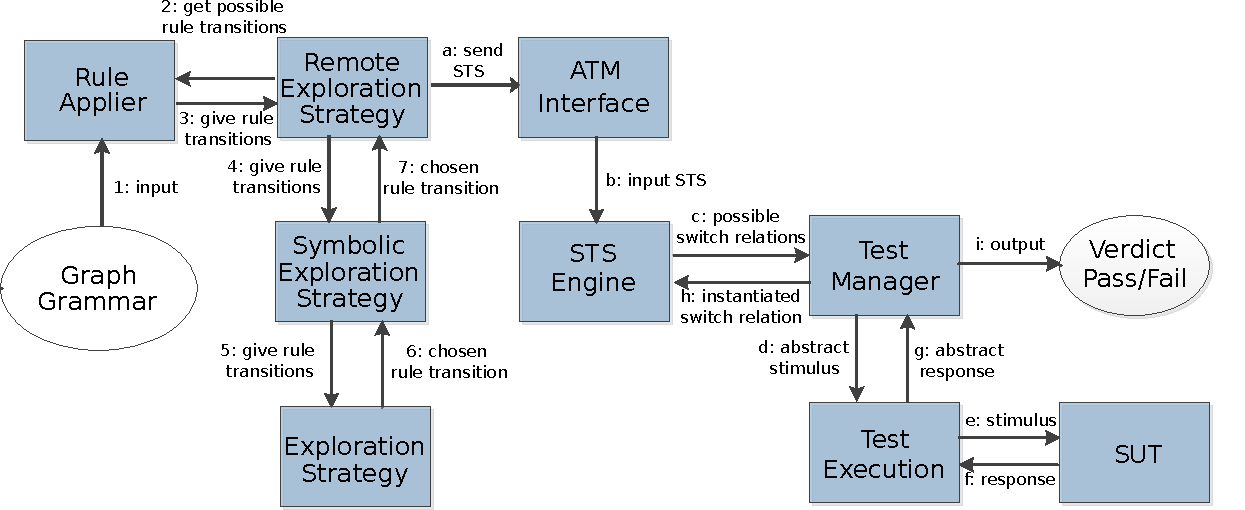
\includegraphics[width=\textwidth]{tooling.pdf}
  \end{center}
  \caption{The GRATiS design: replacing the STS with GROOVE}
  \label{fig:tooling}
\end{figure}

\subsubsection{Problems}\label{sec:problems}
The boardgame example revealed some problems, listed below, for the GRATiS design. These need to be tackled during the design phase of the project. 
\begin{itemize}
  \item Modelling data types such as integers and strings in GROOVE is problematic; the range of possible values has to be given explicitly and cannot be infinite. For example, it would be impossible to extend the die of the boardgame example such that it can throw any integer; each value of an integer would have to be defined separately.
  \item In order to efficiently define transitions with a rule system, sometimes one transition is represented by multiple transitions. In the case of the boardgame example, the \textbf{Player} node moves to the next \textbf{Location} node a number of times equal to the number thrown with the die, as shown in Figure~\ref{fig:statespace_groove1}. A concrete response from the SUT, where the player moves to any location but the next, would need to be translated to a number of 'move' transitions as the abstract response. Otherwise the Test Manager observes this action as erroneous behavior. This translation introduces coupling between the Test Execution component and the specific model. The modularity of these components is therefore lost. %Either the multiple move transitions need to be translated into one abstract label representing the complete movement or the concrete label needs
\end{itemize}

\subsubsection{Coverage}
ATM annotates the locations it has seen and the switch relations it has chosen in the STS. These annotations are needed to calculate the coverage statistics. GRATiS must therefore be able to determine the location of a graph state, by abstracting from the concrete data values in the graph state.

Also, as mentioned in section~\ref{sec:sts_coverage}, the calculation of data coverage for a test run will be implemented in GRATiS.

\subsubsection{Initial design: GRATiS-Min}\label{sec:init_design}
Before the problems in \ref{sec:problems} are tackled and the design of GRATiS implemented, an initial design that minimally achieves the design goal is implemented. This initial design, named GRATiS-Min performs the following steps:
\begin{enumerate}
  \item generate the GTS based on the graph grammar using GROOVE
  \item transform the GTS to an STS with the method described in section~\ref{sec:gts_sts_trafo}
  \item send the STS to ATM
  \item perform the automatic test generation on the STS
\end{enumerate}

There are a number of advantages to GRATiS-Min:
\begin{itemize}
  \item It allows automatic test generation on models which GROOVE is able to fully explore. This has been done on some interesting systems, as described in section~\ref{sec:descriptiongroove}.
  \item It is easy to implement.
  \item It already implements some features of GRATiS, such as the communication between GROOVE and ATM, which makes GRATiS easier to build.
\end{itemize}
And also some disadvantages:
\begin{itemize}
  \item It cannot provide test results on systems with too many states and transitions (for example, due to data values such as integers)
  \item The Test Manager component of ATM cannot use the data values for its test selection strategy, as all values are spread across multiple switch relations. Also, the calculation of location and switch relation coverage statistics on the basic STS will actually reveal the state and transition coverage.
\end{itemize}
The last disadvantage can be solved by providing a better transformation of an LTS to an STS. Constructing such a transformation is a sub-goal of the main design goal, as it improves GRATiS-Min. Therefore, this will be part of the research project.

\subsection{Validation}\label{sec:research_methods_validation}
There are two steps in the validation:
\begin{enumerate}
  \item The boardgame example is tested. A SUT is made for this game and ATM is used to test this game. Then, GRATiS is used to test the boardgame. The results should reveal no errors, fail verdicts or other differences in the output of both tools. An intentional error is then made in the SUT and the process is repeated. Still no errors or differences are expected, but both tools should find the error and give a fail verdict.
  \item Next, the assessment of the strengths and weaknesses of GRATiS is done by applying both tools to several case studies and comparing the results. The case studies are set out first and then the criteria for the comparison are given.
\end{enumerate}

\subsubsection{Case studies}
Three case studies are planned. They are all real-life systems Axini has worked on:
\begin{itemize}
  \item a self-scan register
  \item a navigation system
  \item a health-care system
\end{itemize}  

The self-scan register is a machine that automates the purchase of products at a supermarket. A customer can put his products on a conveyer belt and the system automatically calculates the price of the products. Then the customer pays and gets a receipt. The navigation system is a GPS device with a route planner. It allows a user to enter a destination and the system plans the correct route accordingly from the location of the user. The health-care system is a medical device.

A GTS and an STS will be created for each system. GRATiS and ATM are used for the automatic test generation on these models respectively. Both the model and the test process will then be compared as part of the validation. The next two sections give the criteria for this comparison.

\subsubsection{Objective criteria}
As mentioned in section~\ref{sec:questions}, the criteria for the comparison of ATM and GRATiS are split in two parts. The objective criteria that can be compared are:
\begin{enumerate}
  \item The verdicts: same test cases should give same verdicts. When a verdict is different for the same test case in GRATiS and ATM, this might indicate an error.
  \item The number of bugs found: one tool could generate smarter test-cases and find more bugs.
  \item The coverage: generating smarter test-cases can also lead to a higher coverage.
  \item The test cases generated per second: benchmarks will be done on how fast the tools generate test-cases.
  \item The size of the statespace: benchmarks will be done on how much space the tools use.
\end{enumerate}

\subsubsection{Subjective criteria}
Subjective criteria, such as the maintainability and extendibility of a model, are related to the usability of GTSs versus alternative formalisms, such as STSs. Evaluaiting such criteria requires an extensive experiment with a statistical significant set of human actors. It is out of the scope of this project to perform such an experiment in order to compare two modelling formalisms. In section~\ref{sec:introduction} a motivation is given for the use of GTSs in model-based testing. The qualities of GTSs described there cover the usability of the GTSs.

% the participants are asked to work on one of the case studies. This work entails either:
%\begin{enumerate}
%  \item Extending the model with a new feature
%  \item Finding a bug/error in the SUT/model
%\end{enumerate}
%The following results are then noted and compared:
%\begin{enumerate}
%  \item The time spent on the assignment
%  \item The correctness of the result
%  \item The feelings the participants had with the assignment (how difficult, how much fun, etc.)
%\end{enumerate}

%The results will give insight in the understandibility, maintainability and extendibility of both modelling processes. The results are compiled and presented in the final thesis.

	
	\newpage
	\chapter{Design}
	\newpage
	
	\section{GTS to STS transformation rules}

\subsection{Graph state to location}
Generalized graph states.

\subsection{Rule match to switch relation}
Rule name to gate.

\subsubsection{Variables}
Variable node match from rule to graph state is location variable. Parameterized variable nodes are interaction variables.

\subsubsection{Guard}
NAC expressions over variable nodes in lhs are guards.

\subsubsection{Update}
NAC expressions over variable nodes in rhs are updates.

	\section{Graph grammar exploration}

This section describes a system to transform a graph grammar to an STS without having to explore the entire GTS.

\subsection{Partial matching}
A rule can be checked to see if it \textit{could} match a given graph, if certain elements of the rule were different. In other words, a \textit{partial match} of a rule  can be found on a graph. For example, if the value nodes in a rule match were omitted from the match, the resulting partial match indicates the existence of a rule transition on a graph state with a different value node. Such a partial match therefore indicates the existence of an outgoing switch relation from the location represented by abstracted graph state in the transformed STS. The guard and update mapping can be constructed from the rule, by inspecting which value nodes \textit{would} match the LHS, NACs and RHS. The exploration can then skip graph states which have abstractions isomorphic to graph states already encountered.

This system can potentially lead to an infinitely continuing exploration. An example of a graph grammar where this occurs is shown in Figure~\ref{fig:}. A new graph state is found with each application of the 'add_one' rule. With the partial matching system, this means the GTS and also the transformed STS will expand infinitely. With the normal matching system, this is not the case, as the rule can only be applied three times and then the rule does not match anymore. A solution is to set a modelling constraint on GRATiS, stating that a construction such as the one in Figure~\ref{fig:} may not occur. Section~\ref{sec:reachability} provides another solution to this problem. 

\subsection{Reachability}\label{sec:reachability}
With each new location in the transformed STS the question arises whether that location is reachable from the start location. The MSc thesis of Floor Sietsma "A Case Study in Formal Testing and an Algorithm for Automatic Test Case Generation with Symbolic Transition Systems" gives an algorithm for checking whether a location is reachable. This algorithm works on a specific path, starting from the start location and ending in the location to check. However, with the presence of loops, the number of paths is infinite. A location deemed as unreachable can therefore still be reachable, following a different path. A solution is allow user input for the amount of graph states

	\section{Partial matching}

\subsection{Theory}
Generalizing rule matches.

\subsection{Application}
Using partial matching in an exploration strategy, only the generalized graph states and rule matches are found.

	\section{Reachability}

\subsection{Theory}
MSc thesis Floor Sietsma "A Case Study in Formal Testing and an Algorithm for Automatic Test Case Generation with Symbolic Transition Systems"

\subsection{Application}
Allows halting an exploration strategy when location no longer reachable. Only works for specific path though.

	\section{Pre-testing vs. on-the-fly transformation}

\textit{Pre-testing} transformation is the process of entirely transforming a model before starting test runs. \textit{On-the-fly} transformation is the process of transforming the needed parts of a model while doing a test run.

Explore entire sts + coverage statistics vs. on the fly exploration and no coverage statistics. Being in multiple places at once.
Reachability check in exploration strategy vs. check in on the fly exploration.


	
	\newpage
	\chapter{Validation}
	\newpage
	
	\section{Case Study}\label{sec:case-studies}

GRATiS has been applied to a real-life system Axini has worked on: a self-scan register. The self-scan register is a machine that automates the purchase of products at a supermarket. A customer can put his products on a conveyer belt and the system automatically calculates the price of the products. Then the customer pays and gets a receipt.\marginpar{add figure of machine}.

\subsection{Model}
A graph grammar is created for the self-scan register.add rules as examples. Add isues with modelling.Observation: GG is behavior-specification, was easy to adjust model according to specification. 

\subsection{Model comparison} 
Compare with STS. Nodes-Edges vs. Nodes-Edges? Halstaed's Software science? Compare transformed STS with original STS. Differences? But: transformed STS should be exactly the same! Depends on interpretation, bad-weather testing.


	\section{Benchmarks}

	
	\newpage
	\chapter{Conclusion}
	\newpage
	
	\section{Summary}\label{sec:summary}

	\section{Conclusions}
This report shows the usability of Graph Grammars in model-based testing. The motivation to use GGs is supported by literature, emphasizing the understandibility of graphs and the usefulness of graphs to express system states. Symbolic Transition Systems are a useful formalism which are easily used by computers. This supports using a GG for testers to model a software system and generating the IOSTS from the IOGG for the computer to use during testing. 
The point algebra was shown to be useful for achieving the generation of an IOSTS. The design requirements for GRATiS are all met, because:
\begin{itemize} 
\item the technique proved effective for model-based testing in several example cases and a larger case study
\item coverage can be measured on the generated IOSTS
\item the performance measurements show that the IOSTS can be generated from large models in a negligible time and that the technique scales well
\end{itemize}

Generating the location variables in an STS meant creating an extra definition for GGs, which allowed persistent variables. The definition lets edges to data values to be considered as variables; this was a choice needed to generate the IOSTS. GGs can dynamically add these variables or delete them; something which was frequently desired to obtain the smallest and most intuitive models, but which complicates the generation of the IOSTS. Hence, constraints on GG transformation rules were defined mostly to accomdate the GG variable definition.

One of the example cases, the reservation system, suffered from the constraints the most. This example could not be modelled, because dynamically deleting and creating GG variables was required. The puzzle example on the other hand shows the strength of GGs the most, through simple, intuitive rules opposed to a complicated transition system. This shows that some systems are more suitable to be modelled in GGs than others.

The case study done in this report on the self-scan register shows a real life example of a software system, succefully modelled as an IOGG. Here, the strength of behavioral rules is apparent: instead of state-transition thinking, the graph transformation rules allow each behavioral aspect of a software system to be modelled by one rule. For example, the `not signed on' error, given when the register is in the `not signed on' state. This error can be given in numerous states in the IOSTS, but simply described in the IOGG by matching the state of the register. Additional restrictions of where this rule applies can be easily added to the rule. In state-transition based models, high many states and transitions are often needed to model the same behavior described by one GG rule. This shows that IOGGs are very useful when it comes to changing requirements: only few rules need to be adjusted to accomodate these changes.

Model complexity measurements were done on the IOGGs and IOSTSs of the example cases and case study. This did not reveal a clear difference in overall model complexity. However, it did show that IOGGs generally have more distinct operands, but less overall operators. The first part is due to the labels on nodes and edges, which describe the nature of the nodes and the relation between the nodes; these operands are not present in the IOSTSs. The second part can be explained by the repetition needed in IOSTSs to describe the same behavior as one IOGG rule.

	\section{Future work}
- bedachte measurements die niet gedaan zijn


  \newpage
	\bibliography{bib/bibliography}{}
	\bibliographystyle{plain}
	
	\appendix
  \newpage
\end{document}
